\documentclass[10pt,letterpaper]{article}

\usepackage[T1]{fontenc}
\usepackage{newtxtext,newtxmath}
\usepackage[letterpaper,left=1.5in,right=1.5in,top=0.82in,bottom=0.78in,headheight=14pt]{geometry}
\usepackage{microtype}
\usepackage{amsmath,mathtools,bm}
\usepackage{booktabs,tabularx,longtable,array,multirow}
\usepackage{siunitx}
\usepackage{enumitem}
\usepackage{caption}
\usepackage{fancyhdr}
\usepackage{xcolor}
\usepackage{xurl}
\usepackage{hyperref}
\usepackage{bookmark}
\usepackage[nameinlink,noabbrev]{cleveref}
\usepackage{tikz}
\usetikzlibrary{arrows.meta,positioning,calc,fit}

\definecolor{httblue}{HTML}{315C8A}
\definecolor{httcyan}{HTML}{397C83}
\definecolor{httgreen}{HTML}{42734D}
\definecolor{httamber}{HTML}{A46922}
\definecolor{httred}{HTML}{9B3A36}
\definecolor{httgray}{HTML}{F3F3F3}
\definecolor{citationorange}{HTML}{C55218}

\hypersetup{
  colorlinks=true,
  linkcolor=httblue,
  citecolor=citationorange,
  urlcolor=citationorange,
  pdfauthor={Dhruv Sharma},
  pdftitle={Hyperion Terminal Transformer: Mathematical Architecture and Evaluation Protocol},
  pdfsubject={Prospective mathematical design study for a narrow Terminal artifact-authoring model},
  pdfkeywords={transformer, code generation, constrained decoding, retrieval, verification, calibration}
}

\pagestyle{fancy}
\fancyhf{}
\fancyhead[L]{\small Research project preprint --- not peer reviewed}
\fancyhead[R]{\small HYPERION TERMINAL TRANSFORMER}
\fancyfoot[C]{\small\thepage}
\renewcommand{\headrulewidth}{0.45pt}
\renewcommand{\footrulewidth}{0pt}

\setlength{\parindent}{0pt}
\setlength{\parskip}{4.5pt plus 1pt minus 1pt}
\setlength{\emergencystretch}{2em}
\allowdisplaybreaks[2]
\captionsetup{font=small,labelfont=normalfont,labelsep=colon,justification=justified,singlelinecheck=false}
\setlist{nosep,leftmargin=1.5em,topsep=2pt}
\sisetup{group-separator={,},group-minimum-digits=4,detect-all}

\newcolumntype{Y}{>{\raggedright\arraybackslash}X}
\newcolumntype{L}[1]{>{\raggedright\arraybackslash}p{#1}}
\newcommand{\abbr}[1]{\textsc{\MakeLowercase{#1}}}
\newcommand{\code}[1]{\texttt{\detokenize{#1}}}
\newcommand{\R}{\mathbb{R}}
\newcommand{\E}{\mathbb{E}}
\newcommand{\Prob}{\mathbb{P}}
\newcommand{\1}{\mathbb{1}}
\newcommand{\vect}[1]{\bm{#1}}
\newcommand{\mat}[1]{\bm{#1}}
\newcommand{\given}{\,\middle|\,}
\newcommand{\softmax}{\operatorname{softmax}}
\newcommand{\sigmoid}{\operatorname{sigmoid}}
\newcommand{\clip}{\operatorname{clip}}
\newcommand{\diag}{\operatorname{diag}}
\newcommand{\argmax}{\operatorname*{arg\,max}}
\newcommand{\argmin}{\operatorname*{arg\,min}}
\newcommand{\Risk}{\operatorname{Risk}}
\newcommand{\Coverage}{\operatorname{Coverage}}
\newcommand{\KL}{D_{\mathrm{KL}}}
\newcommand{\NLL}{\operatorname{NLL}}
\newcommand{\ECE}{\operatorname{ECE}}

\tikzset{
  every node/.style={font=\sffamily\scriptsize,align=center},
  httbox/.style={draw=httblue,fill=httblue!6,rounded corners=2pt,minimum height=7mm,minimum width=31mm,inner sep=3pt},
  subbox/.style={draw=black!35,fill=black!3,rounded corners=2pt,minimum height=6mm,inner sep=2.5pt},
  gatebox/.style={draw=httgreen,fill=httgreen!7,rounded corners=2pt,minimum height=7mm,minimum width=31mm,inner sep=3pt},
  warnbox/.style={draw=httamber,fill=httamber!7,rounded corners=2pt,minimum height=7mm,minimum width=31mm,inner sep=3pt},
  rejectbox/.style={draw=httred,fill=httred!7,rounded corners=2pt,minimum height=7mm,minimum width=27mm,inner sep=3pt},
  httarrow/.style={-{Latex[length=2mm]},draw=httblue,thick},
  gatearrow/.style={-{Latex[length=2mm]},draw=httgreen,thick},
  warnarrow/.style={-{Latex[length=2mm]},draw=httamber,thick},
  rejectarrow/.style={-{Latex[length=2mm]},draw=httred,thick}
}

\begin{document}

\begin{center}
  {\LARGE Hyperion Terminal Transformer:\\[2pt]
   A Mathematical Architecture and Evaluation Protocol\par}
  \vspace{8pt}
  {\bfseries Dhruv Sharma\par}
  {Independent Researcher \quad \texttt{dhruvsha.info@gmail.com}\par}
  \vspace{3pt}
  {\itshape Version 2.0 --- 8 August 2026 --- architecture HTT-1.5B-r0\par}
\end{center}

\begin{center}
\begin{minipage}{0.88\linewidth}
\small\itshape
This is a prospective design study and preregistered evaluation protocol.  No Hyperion Terminal
Transformer checkpoint has been trained or evaluated.  Numerical values in this paper are either
algebraic consequences of the proposed dimensions, explicit engineering targets, or results
attributed to prior work.  They are not Hyperion benchmark results.
\end{minipage}
\end{center}

\begin{abstract}
The Hyperion Terminal Transformer (\abbr{HTT}) is a proposed narrow decoder-only language model for
two artifact families: inert Terminal trading-strategy source and declarative Terminal visualizer
specifications.  It is neither a general assistant nor an autonomous trading system.  This paper
specifies the architecture as a falsifiable mathematical object, derives its parameter, operation,
and memory budgets from first principles, and defines the training, retrieval, constrained-decoding,
verification, calibration, and statistical protocols required to evaluate it honestly.

The reference configuration contains 32 transformer blocks, hidden width 2,048, 16 query heads,
four key/value heads, head width 128, SwiGLU width 5,632, a 32,768-token vocabulary, and a maximum
context of 32,768 tokens.  A three-local/one-global attention schedule is repeated eight times.
The core model plus two deterministic rank-64 task lanes contains approximately 1.523 billion
stored parameters; the optional parser-state table raises this to approximately 1.524 billion.
At 32K context and batch size one, the proposed hybrid schedule requires exactly 0.6875 GiB of
BF16 key/value cache under the stated assumptions.  During causal prefill, it reduces attention
score positions by 57.42 percent relative to an all-global schedule; during steady-state decoding,
the corresponding per-query reduction is 65.625 percent.  These are derived quantities, not measured
latency claims.

Accuracy is defined as sealed functional correctness after hard deterministic gates and calibrated
request-level selection.  The protocol reports unconditional accepted yield, selective accuracy,
coverage, compile-at-one, behavioral pass rates, visual fidelity, latency, memory, and energy.  It
separates syntax from semantics, changing private facts from stable skills, and model evidence from
release authority.  The result is a detailed research baseline whose central claims can be rejected
by controlled ablations and future sealed experiments.
\end{abstract}

\section{Introduction and research contributions}

Terminal artifact authoring is a constrained program-synthesis problem.  A useful system must obey
exact software-development-kit (\abbr{SDK}) and schema contracts, remain inside a restricted
capability surface, cite the evidence on which it depends, and emit an artifact that deterministic
tools can compile, render, execute in isolation, and test.  A broad language model may carry billions
of parameters devoted to unrelated knowledge while still failing these domain-specific obligations.
The research question is therefore not ``How small can a chatbot be?'' but rather:

\begin{quote}
What is the smallest reproducible sequence model that can produce correct Terminal artifacts when
current private facts, policy, verification, and release authority remain outside its weights?
\end{quote}

The proposed answer is \abbr{HTT}-1.5B-r0, a dense 1.5B-class decoder with two deterministic task
lanes, selective retrieval, grammar-constrained generation, compiler and renderer feedback,
request-level calibration, and abstention.  The paper makes five research contributions:

\begin{enumerate}
  \item a dimensionally complete mathematical specification of the transformer, conditioning
        features, local/global schedule, and task adapters;
  \item exact parameter and key/value-cache counts plus explicit operation-count approximations;
  \item a domain-limited training program whose losses are normalized by task and artifact region;
  \item an authority-preserving inference protocol in which hard gates cannot be overridden by a
        learned score; and
  \item a sealed evaluation design that measures accuracy after selection, calibration, latency,
        memory, and quantization under paired statistical tests.
\end{enumerate}

The proposal authorizes nothing by itself.  Full pretraining, customer-data use, deployment,
strategy installation, order execution, or a change to the pinned \code{public/} shared-core boundary
requires a separate governance decision.

\subsection{Evidence classes}

Every material statement is one of four kinds:
\begin{description}[style=nextline,leftmargin=0pt]
  \item[Implemented boundary.] Behavior represented by current Hyperion contracts or repository
        documentation.
  \item[Source-reported result.] A finding attributed to cited prior work and not reproduced here.
  \item[Derived quantity.] Arithmetic that follows from declared dimensions and assumptions.
  \item[Research hypothesis.] A proposed choice that must survive a preregistered ablation and sealed
        evaluation.
\end{description}
This separation prevents a cited model's benchmark score or a calculated memory lower bound from
becoming an implied Hyperion result.

\section{Scope, authority, and threat boundary}

\subsection{Allowed purposes}

The coordinator, not the model, selects exactly one purpose:
\begin{itemize}
  \item \code{STRATEGY}: author or repair inert C\# or DAXQ strategy artifacts inside the restricted
        Terminal strategy surface; or
  \item \code{VISUALIZER}: author or repair a declarative visualizer specification that a deterministic
        compiler may later translate into an allowlisted renderer.
\end{itemize}
The model may explain fields and diagnostics of the artifact being produced.  It is not designed for
news, biography, open-domain programming, discretionary trade calls, portfolio allocation, broker
operations, credential handling, arbitrary desktop automation, or unrestricted web access.

The current strategy result is a \code{CoordinatorStrategySourceArtifact}.  It binds objectives,
evidence identifiers, role outputs, exact file hashes, and source files.  The future visualizer shape,
\code{hyperion-terminal-visualizer/v1}, is deliberately non-executable: it contains allowlisted data
sources, transformations, panes, series, axes, legends, interactions, accessibility labels, and
bounded update behavior, but no network, filesystem, reflection, process, package, native-code,
broker, or credential field.

\subsection{What ``Terminal-only knowledge'' can mean}

No executable code model can be proven to contain literally zero outside knowledge: C\#, JSON,
mathematics, and natural language already contain general regularities.  The defensible operational
claim is narrower:
\begin{enumerate}
  \item admitted weight-training records are restricted by rights, domain, and provenance;
  \item mutable private APIs and conventions are supplied through revocable, versioned retrieval;
  \item out-of-scope requests are rejected before generation or mapped to a refusal artifact;
  \item grammar masks expose only the allowed artifact language;
  \item compilers, renderers, tests, and policy engines determine executable validity; and
  \item the served model has no direct network, filesystem, package, broker, or release authority.
\end{enumerate}

\begin{figure}[t]
  \centering
  \resizebox{\linewidth}{!}{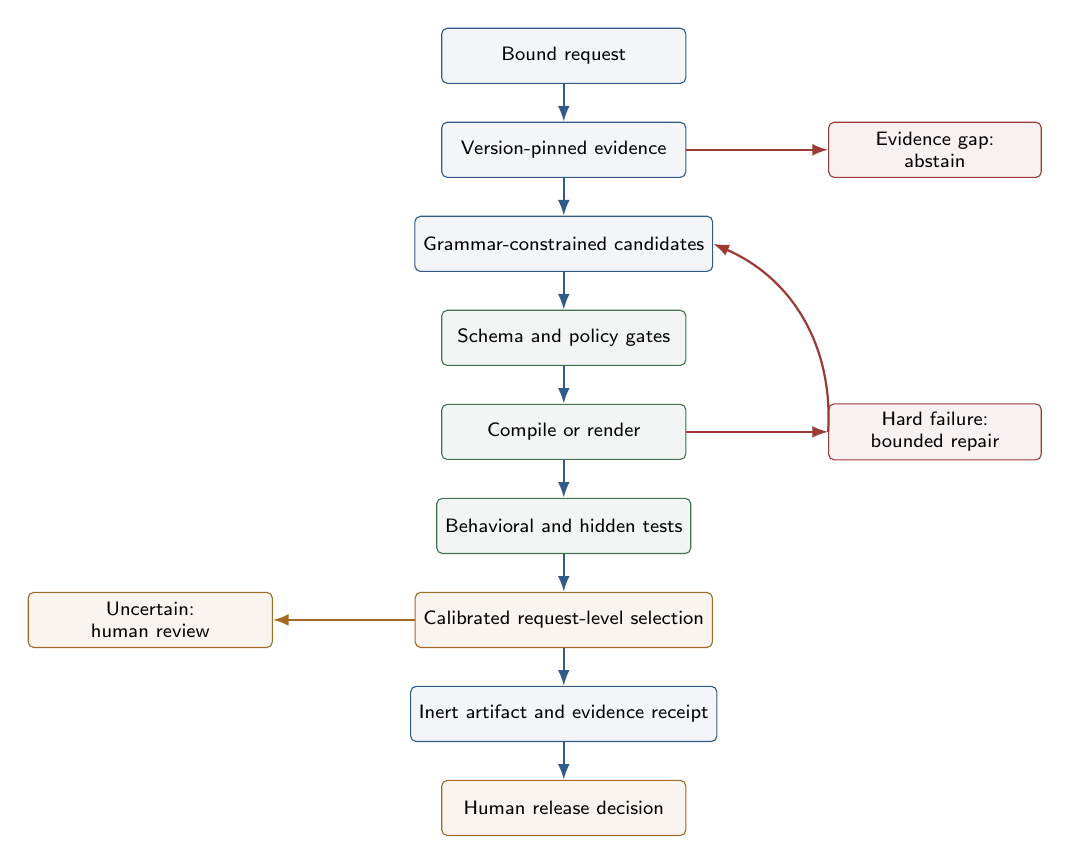
\begin{tikzpicture}[node distance=4.8mm and 11mm]
  \node[httbox] (request) {Bound request};
  \node[httbox, below=of request] (evidence) {Version-pinned evidence};
  \node[httbox, below=of evidence] (generate) {Grammar-constrained candidates};
  \node[gatebox, below=of generate] (schema) {Schema and policy gates};
  \node[gatebox, below=of schema] (compile) {Compile or render};
  \node[gatebox, below=of compile] (tests) {Behavioral and hidden tests};
  \node[warnbox, below=of tests] (select) {Calibrated request-level selection};
  \node[httbox, below=of select] (artifact) {Inert artifact and evidence receipt};
  \node[warnbox, below=of artifact] (human) {Human release decision};
  \node[rejectbox, right=18mm of evidence] (abstain) {Evidence gap:\\abstain};
  \node[rejectbox, right=18mm of compile] (repair) {Hard failure:\\bounded repair};
  \node[warnbox, left=18mm of select] (review) {Uncertain:\\human review};
  \draw[httarrow] (request) -- (evidence);
  \draw[httarrow] (evidence) -- (generate);
  \draw[httarrow] (generate) -- (schema);
  \draw[httarrow] (schema) -- (compile);
  \draw[httarrow] (compile) -- (tests);
  \draw[httarrow] (tests) -- (select);
  \draw[httarrow] (select) -- (artifact);
  \draw[httarrow] (artifact) -- (human);
  \draw[rejectarrow] (evidence) -- (abstain);
  \draw[rejectarrow] (compile) -- (repair);
  \draw[rejectarrow] (repair.west) to[bend right=35] (generate.east);
  \draw[warnarrow] (select) -- (review);
\end{tikzpicture}
}
  \caption{\textbf{Authority-preserving artifact lifecycle.} Generation can repair or abstain, but a
  learned score never bypasses a hard deterministic gate.}
  \label{fig:lifecycle}
\end{figure}

\section{Notation and abbreviations}

\subsection{Mathematical conventions}

Vectors are bold lowercase, matrices are bold uppercase, and all token representations are row
vectors unless an equation explicitly transposes them.  Natural logarithms are used throughout.
A multiply-add is counted as two floating-point operations in operation estimates.  Parameter counts
exclude biases unless stated.  Memory uses bytes, decimal GB ($10^9$ bytes), and binary GiB
($2^{30}$ bytes) distinctly.  Context length and evaluation sample size use different symbols.

\begin{longtable}{@{}L{0.20\linewidth}L{0.25\linewidth}L{0.47\linewidth}@{}}
\caption{Principal mathematical symbols.}\label{tab:symbols}\\
\toprule
Symbol & Domain or shape & Meaning \\
\midrule
\endfirsthead
\toprule Symbol & Domain or shape & Meaning \\
\midrule
\endhead
$|\mathcal V|$ & $\mathbb N$ & tokenizer vocabulary size \\
$N_{\mathrm{ctx}}$ & $\mathbb N$ & current context length in tokens \\
$N_{\mathrm{eval}}$ & $\mathbb N$ & number of evaluation requests \\
$d$ & $\mathbb N$ & hidden width \\
$d_h$ & $\mathbb N$ & attention-head width \\
$d_{\mathrm{ff}}$ & $\mathbb N$ & SwiGLU intermediate width \\
$n_{\mathrm{layer}}$ & $\mathbb N$ & decoder-block count \\
$h_q,h_{\mathrm{kv}}$ & $\mathbb N$ & query-head and key/value-head counts \\
$W$ & $\mathbb N$ & local attention window, including the current token \\
$\mat Q,\mat K,\mat V$ & matrices & attention queries, keys, and values \\
$\ell$ & $\{\mathrm{strategy},\mathrm{visualizer}\}$ & server-selected task lane \\
$r_a$ & $\mathbb N$ & task-adapter rank \\
$K_{\mathrm{cand}}$ & $\mathbb N$ & candidates generated per request \\
$\tau$ & $[0,1]$ & post-selection acceptance threshold \\
$\mathcal L$ & $\mathbb R_{\ge0}$ & a loss; subscripts identify the objective \\
$P$ & $\mathbb N$ & parameter count \\
$M$ & bytes & memory quantity \\
$B$ & $\mathbb N$ & inference batch size \\
\bottomrule
\end{longtable}

\subsection{Abbreviation glossary}

Code typography is reserved for literal program identifiers such as \code{OnBar},
\code{schemaVersion}, or \code{STRATEGY}.  Mathematical and engineering abbreviations are ordinary
small-cap text.

\begin{longtable}{@{}L{0.21\linewidth}L{0.73\linewidth}@{}}
\caption{Abbreviations used in the paper.}\label{tab:abbreviations}\\
\toprule Abbreviation & Meaning \\
\midrule
\endfirsthead
\toprule Abbreviation & Meaning \\
\midrule
\endhead
\abbr{HTT} & Hyperion Terminal Transformer \\
\abbr{LLM} & large language model \\
\abbr{NTP}/\abbr{MTP} & next-token prediction / multi-token prediction \\
\abbr{MHA}/\abbr{MQA}/\abbr{GQA} & multi-head / multi-query / grouped-query attention \\
\abbr{KV}/\abbr{QK} & key--value / query--key \\
\abbr{RMSNorm}/\abbr{RoPE} & root-mean-square normalization / rotary position encoding \\
\abbr{FFN}/\abbr{GLU}/\abbr{SwiGLU} & feed-forward network / gated linear unit / SiLU-gated GLU \\
\abbr{FIM} & fill in the middle \\
\abbr{BPE} & byte-pair encoding \\
\abbr{RAG} & retrieval-augmented generation \\
\abbr{SFT}/\abbr{DPO} & supervised fine-tuning / direct preference optimization \\
\abbr{RL}/\abbr{RLVR}/\abbr{GRPO}/\abbr{RLOO} & reinforcement learning / reinforcement learning
with verifiable rewards / group-relative policy optimization / reinforce leave-one-out \\
\abbr{KL}/\abbr{NLL}/\abbr{ECE} & Kullback--Leibler divergence / negative log likelihood /
expected calibration error \\
\abbr{IR}/\abbr{AST}/\abbr{IL} & intermediate representation / abstract syntax tree /
intermediate language \\
\abbr{SDK}/\abbr{API}/\abbr{DSL} & software development kit / application programming interface /
domain-specific language \\
\abbr{BF16}/\abbr{FP8}/\abbr{INT8}/\abbr{INT4} & numeric storage or arithmetic formats \\
\abbr{GPU}/\abbr{CUDA}/\abbr{IO} & graphics processor / NVIDIA compute platform / input--output \\
\abbr{AWQ}/\abbr{GPTQ} & activation-aware weight quantization / post-training weight quantization \\
\abbr{MoE}/\abbr{BLT} & mixture of experts / byte latent transformer \\
DAXQ & Hyperion's restricted numeric strategy language; no expansion is assumed \\
\bottomrule
\end{longtable}

\section{Formal task and artifact model}

Let a request be
\begin{equation}
  \mathcal R = (u,\ell,s,v,\mathcal E,\mathcal C,\mathcal B),
  \label{eq:request}
\end{equation}
where $u$ is the bounded user objective, $\ell$ is the server-selected task lane, $s$ is the output
schema identity, $v$ is the Terminal/SDK version, $\mathcal E$ is an authorized evidence set,
$\mathcal C$ is the deterministic capability policy, and $\mathcal B$ contains token, tool, time,
and candidate budgets.  The model emits a candidate artifact $y$ and non-authoritative diagnostics.
The coordinator recomputes all hashes, identities, and authority fields.

Define hard predicates $g_m(y,\mathcal R)\in\{0,1\}$ for schema validity, policy, compilation or
rendering, resource limits, prohibited capabilities, and required behavioral tests.  Hard feasibility
is
\begin{equation}
  H(y,\mathcal R)=\prod_{m=1}^{M_g} g_m(y,\mathcal R).
  \label{eq:hard-feasible}
\end{equation}
No learned score can change a zero in this product into a one.  The feasible set for request $j$ is
\begin{equation}
  \mathcal F_j=\{,i\in\{1,\ldots,K_{\mathrm{cand}}\}:H(y_{ji},\mathcal R_j)=1\,\}.
  \label{eq:feasible-set}
\end{equation}
If $\mathcal F_j=\varnothing$, the system repairs within a fixed budget or abstains.  Human release
is a later decision outside the model.

\section{Transformer foundations and complete block equations}

\subsection{Token representation and immutable conditioning}

For tokens $t_1,\ldots,t_{N_{\mathrm{ctx}}}\in\mathcal V$, let
$\mat E_{\mathrm{tok}}\in\R^{|\mathcal V|\times d}$ be the tied input/output embedding.  The input
to position $i$ is
\begin{align}
  \vect x_i^{(0)}
  &= \mat E_{\mathrm{tok}}[t_i]
   + \vect e^{\mathrm{role}}_{r_i}
   + \vect e^{\mathrm{task}}_{\ell}
   + \vect e^{\mathrm{schema}}_{s}
   + \delta_{\mathrm{parser}}\mat E_{\mathrm{grammar}}[g_i],
  \label{eq:input-embedding}\\
  \mat X^{(0)}
  &= [\vect x_1^{(0)};\ldots;\vect x_{N_{\mathrm{ctx}}}^{(0)}]
  \in\R^{N_{\mathrm{ctx}}\times d}.
\end{align}
Here $\delta_{\mathrm{parser}}\in\{0,1\}$ controls the optional parser-state feature and
$g_i$ is computed only from the already emitted prefix, so it cannot leak future tokens.  Absolute
position is not added to \cref{eq:input-embedding}; \abbr{RoPE} acts on queries and keys.

\subsection{Why dot-product attention is scaled}

For one head, take
\begin{equation}
  \mat Q=\mat X\mat W_Q,\qquad
  \mat K=\mat X\mat W_K,\qquad
  \mat V=\mat X\mat W_V,
  \label{eq:qkv}
\end{equation}
with $\mat Q,\mat K,\mat V\in\R^{N_{\mathrm{ctx}}\times d_h}$.  Suppose, only for the
variance calculation, that components $q_m$ and $k_m$ are independent, mean zero, and have variance
$\sigma^2$.  Then
\begin{align}
  \E[\vect q^\top\vect k]
  &=\sum_{m=1}^{d_h}\E[q_mk_m]=0,\\
  \operatorname{Var}(\vect q^\top\vect k)
  &=\sum_{m=1}^{d_h}\operatorname{Var}(q_mk_m)
    =d_h\sigma^4.
  \label{eq:dot-var}
\end{align}
Without scaling, score variance grows linearly with head width and pushes the softmax toward saturated
probabilities.  Dividing by $\sqrt{d_h}$ yields
\begin{equation}
  \operatorname{Var}\!\left(\frac{\vect q^\top\vect k}{\sqrt{d_h}}\right)=\sigma^4,
  \label{eq:scaled-var}
\end{equation}
which is independent of $d_h$ under the stated approximation.  The masked attention matrix is
\begin{align}
  \mat S &= \frac{\mat Q\mat K^\top}{\sqrt{d_h}}+\mat M,\\
  M_{ij} &=
  \begin{cases}
    0, & j\le i\text{ and }j\text{ is inside the layer's window},\\
    -\infty, & \text{otherwise},
  \end{cases}\\
  \operatorname{Attn}(\mat Q,\mat K,\mat V)
  &=\softmax_{\mathrm{row}}(\mat S)\mat V.
  \label{eq:sdpa}
\end{align}
The mathematical mask is $-\infty$; an implementation uses the most negative safe value for the
chosen kernel and dtype.  Exact-attention kernels may reorder floating-point operations while
remaining algorithmically equivalent to \cref{eq:sdpa}; ``exact'' does not mean bitwise identical.

\subsection{Multi-head and grouped-query attention}

With $h_q$ query heads, the output is
\begin{equation}
  \operatorname{MHA}(\mat X)
  =\operatorname{Concat}(\mat O_1,\ldots,\mat O_{h_q})\mat W_O,
  \qquad \mat W_O\in\R^{h_qd_h\times d}.
  \label{eq:mha}
\end{equation}
Ordinary multi-head attention has $h_q$ key and value heads.  Multi-query attention has one.
Grouped-query attention (\abbr{GQA}) chooses $h_{\mathrm{kv}}\mid h_q$ and group size
\begin{equation}
  g=\frac{h_q}{h_{\mathrm{kv}}},\qquad
  \kappa(a)=1+\left\lfloor\frac{a-1}{g}\right\rfloor,
  \label{eq:gqa-map}
\end{equation}
so query head $a$ uses key/value head $\kappa(a)$.  For bias-free projections,
\begin{align}
  P_Q &= d(h_qd_h), & P_K&=d(h_{\mathrm{kv}}d_h),\\
  P_V &= d(h_{\mathrm{kv}}d_h), & P_O&=(h_qd_h)d.
\end{align}
Because $h_qd_h=d$ in HTT,
\begin{equation}
  P_{\mathrm{attn}}
  =2d^2+2d h_{\mathrm{kv}}d_h.
  \label{eq:attn-params}
\end{equation}
For $d=2{,}048$, $h_q=16$, $h_{\mathrm{kv}}=4$, and $d_h=128$, this is
\begin{align}
  P_{\mathrm{attn}}
  &=2(2{,}048)^2+2(2{,}048)(4)(128)\\
  &=8{,}388{,}608+2{,}097{,}152\\
  &=10{,}485{,}760
  \quad\text{parameters per layer}.
  \label{eq:attn-params-numeric}
\end{align}

\subsection{Rotary position encoding}

Let $m\in\{0,\ldots,d_h/2-1\}$ index coordinate pairs and define frequency
\begin{equation}
  \omega_m=b^{-2m/d_h},
  \label{eq:rope-frequency}
\end{equation}
where $b$ is the selected \abbr{RoPE} base.  At position $p$, pair $m$ is rotated by
\begin{equation}
  \mat R_m(p)=
  \begin{bmatrix}
    \cos(p\omega_m)&-\sin(p\omega_m)\\
    \sin(p\omega_m)& \cos(p\omega_m)
  \end{bmatrix}.
  \label{eq:rope-pair}
\end{equation}
The full $\mat R(p)$ is block diagonal with the $d_h/2$ pair matrices.  Orthogonality and angle
addition give
\begin{align}
  \mat R_m(p)^\top\mat R_m(r)
  &=\mat R_m(-p)\mat R_m(r)\\
  &=\mat R_m(r-p).
\end{align}
Therefore the rotated dot product is
\begin{equation}
  (\mat R(p)\vect q)^\top(\mat R(r)\vect k)
  =\vect q^\top\mat R(r-p)\vect k,
  \label{eq:rope-relative}
\end{equation}
which depends on relative displacement $r-p$ while retaining content-dependent $\vect q$ and
$\vect k$ \cite{su2021roformer}.

\subsection{RMSNorm, QK-Norm, and the pre-normalized residual path}

For $\vect x\in\R^d$, learned gain $\vect\gamma\in\R^d$, and $\epsilon>0$, define
\begin{align}
  \rho(\vect x)&=\sqrt{\frac{1}{d}\vect x^\top\vect x+\epsilon},\\
  \operatorname{RMSNorm}(\vect x)
  &=\vect\gamma\odot\frac{\vect x}{\rho(\vect x)}.
  \label{eq:rmsnorm}
\end{align}
The Jacobian exposes both the direct scaling path and the rank-one normalization correction:
\begin{equation}
  \frac{\partial\operatorname{RMSNorm}(\vect x)}{\partial\vect x}
  =\diag(\vect\gamma)
   \left[
     \frac{\mat I}{\rho(\vect x)}
     -\frac{\vect x\vect x^\top}{d\,\rho(\vect x)^3}
   \right].
  \label{eq:rmsnorm-jacobian}
\end{equation}
Ignoring $\epsilon$, multiplying $\vect x$ by a positive scalar cancels between numerator and
denominator, explaining the normalization's approximate scale invariance \cite{zhang2019rmsnorm}.

HTT additionally normalizes each query and key head across its $d_h$ coordinates before \abbr{RoPE}:
\begin{equation}
  \widehat{\vect q}_{ia}=\operatorname{RMSNorm}_{q}(\vect q_{ia}),\qquad
  \widehat{\vect k}_{ib}=\operatorname{RMSNorm}_{k}(\vect k_{ib}).
  \label{eq:qknorm}
\end{equation}
The reference count assumes one $d_h$-element gain shared across query heads and one shared across
key heads, adding $2d_h=256$ parameters per block.  Per-head gains are a different, larger model and
must be counted separately.

For block function $F_l$, pre-normalization uses
\begin{equation}
  \vect x_{l+1}=\vect x_l+F_l(\operatorname{RMSNorm}(\vect x_l)).
  \label{eq:prenorm}
\end{equation}
Its local Jacobian has an explicit identity term,
\begin{equation}
  \frac{\partial\vect x_{l+1}}{\partial\vect x_l}
  =\mat I+\mat J_{F_l}\mat J_{\mathrm{RMS},l},
  \label{eq:prenorm-jacobian}
\end{equation}
so the residual stream contains a depth-independent identity route.  This does not guarantee stable
training, but it avoids forcing every gradient through a terminal normalization transform.

\subsection{SwiGLU and the width-matching derivation}

For row input $\vect x\in\R^d$, define
\begin{align}
  \vect u&=\vect x\mat W_u,&
  \vect g&=\vect x\mat W_g,\\
  \operatorname{SiLU}(z)&=z\sigmoid(z),&
  \operatorname{SwiGLU}(\vect x)
  &=\left[\operatorname{SiLU}(\vect g)\odot\vect u\right]\mat W_d,
  \label{eq:swiglu}
\end{align}
where $\mat W_u,\mat W_g\in\R^{d\times d_{\mathrm{ff}}}$ and
$\mat W_d\in\R^{d_{\mathrm{ff}}\times d}$.  Its bias-free parameter count is
\begin{equation}
  P_{\mathrm{ffn}}=3dd_{\mathrm{ff}}.
  \label{eq:ffn-params}
\end{equation}
A conventional two-matrix feed-forward network of width $4d$ contains
$d(4d)+(4d)d=8d^2$ parameters.  Matching the SwiGLU count gives
\begin{align}
  3dd_{\mathrm{ff}}&\approx8d^2,\\
  d_{\mathrm{ff}}&\approx\frac{8d}{3}.
  \label{eq:ffn-match}
\end{align}
At $d=2{,}048$, the exact rule yields $5{,}461\tfrac{1}{3}$.  The proposed tensor-friendly value
$5{,}632$ is $170\tfrac{2}{3}$ units, or 3.125 percent, larger.  Consequently
\begin{equation}
  P_{\mathrm{ffn}}=3(2{,}048)(5{,}632)=34{,}603{,}008.
  \label{eq:ffn-numeric}
\end{equation}
SwiGLU is adopted as a candidate supported by prior matched-compute language-model results, not as a
guaranteed HTT improvement \cite{shazeer2020glu}.

\subsection{Complete decoder block}

For layer $l$, suppressing dropout because the serving graph is deterministic,
\begin{align}
  \mat A_l
  &=\operatorname{GQA}_l\!\left(\operatorname{RMSNorm}_{l,1}(\mat X_l);\mat M_l\right),\\
  \widetilde{\mat X}_l
  &=\mat X_l+\mat A_l+\mathcal A^{\mathrm{attn}}_{l,\ell}(\mat X_l),\\
  \mat F_l
  &=\operatorname{SwiGLU}_l\!\left(\operatorname{RMSNorm}_{l,2}(\widetilde{\mat X}_l)\right),\\
  \mat X_{l+1}
  &=\widetilde{\mat X}_l+\mat F_l
    +\mathcal A^{\mathrm{ffn}}_{l,\ell}(\widetilde{\mat X}_l).
  \label{eq:full-block}
\end{align}
The task-adapter maps $\mathcal A$ are zero outside the top 12 blocks.  A final RMSNorm produces
$\mat H$, and tied logits are
\begin{equation}
  \mat Z=\mat H\mat E_{\mathrm{tok}}^\top.
  \label{eq:tied-logits}
\end{equation}

\section{Proposed HTT-1.5B-r0 architecture}

\begin{table}[t]
\centering
\caption{Reference architecture.  Every value is a hypothesis until an ablation establishes it.}
\label{tab:architecture}
\small
\begin{tabularx}{\linewidth}{@{}L{0.27\linewidth}L{0.19\linewidth}Y@{}}
\toprule
Component & Proposed value & Required comparison \\
\midrule
Decoder blocks & 32 & 24 and 36 blocks at matched active parameters \\
Hidden width $d$ & 2,048 & 1,792 and 2,304 \\
Query / key-value heads & 16 / 4 & $h_{\mathrm{kv}}\in\{1,2,8,16\}$ \\
Head width $d_h$ & 128 & 64 and 128 at matched hidden width \\
SwiGLU width $d_{\mathrm{ff}}$ & 5,632 & 5,504 and 6,144 \\
Vocabulary $|\mathcal V|$ & 32,768 & 16K, 48K, and inherited large tokenizer \\
Maximum context & 32,768 & 8K and 16K operating points \\
Local window $W$ & 4,096 & 2K, 8K, and all-global \\
Global schedule & every fourth block & every sixth block and all-global \\
Task lanes & rank 64 in top 12 blocks & shared trunk and separate models \\
Training baseline & BF16 & FP8 only after numerical parity \\
\bottomrule
\end{tabularx}
\end{table}

\begin{figure}[t]
  \centering
  \resizebox{\linewidth}{!}{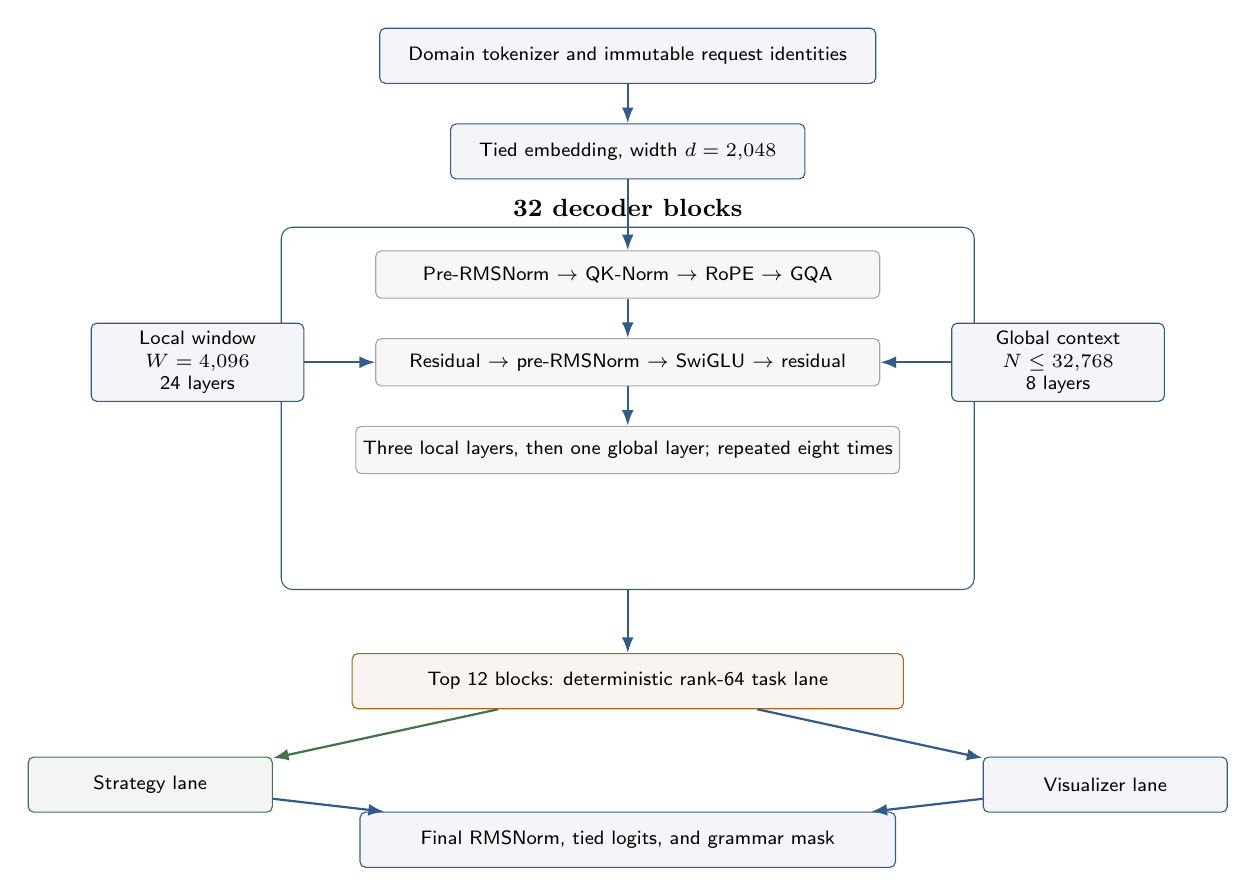
\begin{tikzpicture}[node distance=5mm and 8mm]
  \node[httbox, minimum width=63mm] (tokens) {Domain tokenizer and immutable request identities};
  \node[httbox, below=of tokens, minimum width=45mm] (embed) {Tied embedding, width $d=2{,}048$};
  \node[draw=httblue, rounded corners, below=6mm of embed, minimum width=88mm,
        minimum height=46mm, fill=white, label={[font=\bfseries\small]above:32 decoder blocks}] (stack) {};
  \node[subbox, below=9mm of embed, minimum width=64mm] (attn) {Pre-RMSNorm $\rightarrow$ QK-Norm $\rightarrow$ RoPE $\rightarrow$ GQA};
  \node[subbox, below=of attn, minimum width=64mm] (ffn) {Residual $\rightarrow$ pre-RMSNorm $\rightarrow$ SwiGLU $\rightarrow$ residual};
  \node[subbox, below=of ffn, minimum width=64mm] (schedule) {Three local layers, then one global layer; repeated eight times};
  \node[httbox, left=9mm of ffn, minimum width=27mm] (local) {Local window\\$W=4{,}096$\\24 layers};
  \node[httbox, right=9mm of ffn, minimum width=27mm] (global) {Global context\\$N\le 32{,}768$\\8 layers};
  \node[warnbox, below=8mm of stack, minimum width=70mm] (lanes) {Top 12 blocks: deterministic rank-64 task lane};
  \node[gatebox, below left=6mm and 10mm of lanes] (strategy) {Strategy lane};
  \node[httbox, below right=6mm and 10mm of lanes] (visual) {Visualizer lane};
  \node[httbox, below=13mm of lanes, minimum width=68mm] (logits) {Final RMSNorm, tied logits, and grammar mask};
  \draw[httarrow] (tokens) -- (embed);
  \draw[httarrow] (embed) -- (attn);
  \draw[httarrow] (attn) -- (ffn);
  \draw[httarrow] (ffn) -- (schedule);
  \draw[httarrow] (local) -- (ffn);
  \draw[httarrow] (global) -- (ffn);
  \draw[httarrow] (stack) -- (lanes);
  \draw[gatearrow] (lanes) -- (strategy);
  \draw[httarrow] (lanes) -- (visual);
  \draw[httarrow] (strategy) -- (logits);
  \draw[httarrow] (visual) -- (logits);
\end{tikzpicture}
}
  \caption{\textbf{HTT-1.5B-r0 computational graph.}  The task lane is chosen by the coordinator,
  never by a learned router.  Grammar masking and deterministic tools remain outside the backbone.}
  \label{fig:architecture}
\end{figure}

\subsection{Local/global attention schedule}

Blocks follow three local layers followed by one global layer, repeated eight times.  A local query at
position $i$ can attend to keys
\begin{equation}
  j\in\{\max(1,i-W+1),\ldots,i\}.
  \label{eq:local-window}
\end{equation}
Because the window includes the current token, one local layer expands the maximum causal receptive
span by $W-1$.  Ignoring optimization and attenuation, after $k$ consecutive local layers the exact
maximum span is
\begin{equation}
  R_k=1+k(W-1).
  \label{eq:local-receptive-field}
\end{equation}
A global layer directly connects every position to the full causal prefix.  The 3:1 schedule is more
global than the 5:1 pattern reported for Gemma 3 because cross-file references and compiler repair
may need frequent long-range exchange; that rationale is a hypothesis and the 5:1 schedule remains a
mandatory challenger \cite{jiang2023mistral,gemma2025}.

\subsection{Exact causal score counts}

For one all-global causal layer with context $N=N_{\mathrm{ctx}}$, the number of unmasked query--key
positions is the triangular sum
\begin{equation}
  S_G(N)=\sum_{i=1}^{N}i=\frac{N(N+1)}{2}.
  \label{eq:global-score-count}
\end{equation}
For a local layer with window $W\le N$,
\begin{align}
  S_L(N,W)
  &=\sum_{i=1}^{N}\min(i,W)\\
  &=\sum_{i=1}^{W}i+\sum_{i=W+1}^{N}W\\
  &=\frac{W(W+1)}{2}+(N-W)W\\
  &=NW-\frac{W(W-1)}{2}.
  \label{eq:local-score-count}
\end{align}
With $L_G=8$ global and $L_L=24$ local blocks, the causal-prefill score ratio relative to 32
all-global blocks is
\begin{equation}
  R_{\mathrm{prefill}}(N,W)
  =\frac{L_GS_G(N)+L_LS_L(N,W)}{(L_G+L_L)S_G(N)}.
  \label{eq:prefill-ratio}
\end{equation}
At $N=32{,}768$ and $W=4{,}096$,
\begin{align}
  S_G &= 536{,}887{,}296,\\
  S_L &= 125{,}831{,}168,\\
  S_{\mathrm{hybrid}}
      &=8S_G+24S_L=7{,}315{,}046{,}400,\\
  S_{\mathrm{all\ global}}
      &=32S_G=17{,}180{,}393{,}472,\\
  R_{\mathrm{prefill}}&=0.4257787467.
\end{align}
Thus the exact causal score-position reduction is
\begin{equation}
  1-R_{\mathrm{prefill}}=0.5742212533,
\end{equation}
or 57.42 percent.  The earlier rectangular approximation
$[8N+24W]/(32N)=0.34375$ describes one steady-state decode query at full context, not causal prefill.
For that decode regime, the score-position reduction is 65.625 percent.  Keeping these regimes
separate prevents an inference-only ratio from being reported as a training-compute result.

\subsection{Deterministic low-rank task lanes}

For row vector $\vect x\in\R^d$, adapter rank $r_a=64$, and lane $\ell$, define
\begin{equation}
  \mathcal A_{l,\ell}(\vect x)
  =\operatorname{SiLU}(\vect x\mat A_{l,\ell})\mat B_{l,\ell},
  \quad
  \mat A_{l,\ell}\in\R^{d\times r_a},\quad
  \mat B_{l,\ell}\in\R^{r_a\times d}.
  \label{eq:adapter}
\end{equation}
There are two adapter positions in each of the top 12 blocks.  With no biases and no learned scalar,
one lane contains
\begin{align}
  P_{\mathrm{lane}}
  &=12\text{ blocks}\times2\text{ positions}\times(2dr_a)\\
  &=12\times2\times2\times2{,}048\times64\\
  &=6{,}291{,}456.
  \label{eq:lane-count}
\end{align}
Initializing every $\mat B_{l,\ell}=\mat 0$ makes the initial network exactly equal to the shared
trunk while allowing gradients into $\mat B$.  Merely saying ``near zero'' would not establish exact
equality.  A learned scalar per adapter would add 24 parameters per lane and must be declared in the
executable manifest.

The lane is an inductive bias, not an authority mechanism.  It cannot select a schema, retrieve
evidence, grant a capability, or release an artifact.  A learned mixture-of-experts router is deferred
until the dense baseline is reproducible because sparse routing introduces expert balance,
communication, quantization, storage, and rollback questions \cite{shazeer2017moe,fedus2022switch}.

\section{Parameter-count derivation}

This section derives every reference-graph count from matrix shapes.  Let
\begin{equation}
  |\mathcal V|=32{,}768,\quad d=2{,}048,\quad n_{\mathrm{layer}}=32,
  \quad h_q=16,\quad h_{\mathrm{kv}}=4,\quad d_h=128,
  \quad d_{\mathrm{ff}}=5{,}632.
\end{equation}

\subsection{Embedding, block, and identity parameters}

The tied token embedding/output matrix contributes
\begin{equation}
  P_{\mathrm{embed}}=|\mathcal V|d=32{,}768\times2{,}048=67{,}108{,}864.
  \label{eq:embedding-count}
\end{equation}
From \cref{eq:attn-params-numeric,eq:ffn-numeric}, plus two $d$-element RMSNorm gains and two
shared $d_h$-element QK-Norm gains,
\begin{align}
  P_{\mathrm{block}}
  &=P_{\mathrm{attn}}+P_{\mathrm{ffn}}+2d+2d_h\\
  &=10{,}485{,}760+34{,}603{,}008+4{,}096+256\\
  &=45{,}093{,}120,\\
  P_{\mathrm{blocks}}
  &=32P_{\mathrm{block}}=1{,}442{,}979{,}840.
  \label{eq:block-count}
\end{align}
The final RMSNorm adds $d=2{,}048$ parameters.

Identity embeddings must be auditable rather than represented by an unexplained approximation.  The
reference budget reserves 16 identity rows: eight coordinator roles, two task lanes, four schema
families, and two boundary states.  Therefore
\begin{equation}
  P_{\mathrm{identity}}=d(8+2+4+2)=2{,}048\times16=32{,}768.
  \label{eq:identity-count}
\end{equation}
Changing these cardinalities changes the count.  The core shared base is
\begin{align}
  P_{\mathrm{base}}
  &=P_{\mathrm{embed}}+P_{\mathrm{blocks}}+d+P_{\mathrm{identity}}\\
  &=67{,}108{,}864+1{,}442{,}979{,}840+2{,}048+32{,}768\\
  &=1{,}510{,}123{,}520.
  \label{eq:base-count}
\end{align}

\subsection{Stored and active totals}

Two task lanes add
\begin{equation}
  P_{\mathrm{lanes}}=2P_{\mathrm{lane}}=12{,}582{,}912.
\end{equation}
The core stored total and one-lane active total are
\begin{align}
  P_{\mathrm{stored,core}}
  &=P_{\mathrm{base}}+P_{\mathrm{lanes}}
    =1{,}522{,}706{,}432,\\
  P_{\mathrm{active,core}}
  &=P_{\mathrm{base}}+P_{\mathrm{lane}}
    =1{,}516{,}414{,}976.
  \label{eq:core-totals}
\end{align}
The optional parser-state table has 512 states:
\begin{equation}
  P_{\mathrm{parser}}=512d=1{,}048{,}576.
\end{equation}
Consequently
\begin{align}
  P_{\mathrm{stored,parser}}&=1{,}523{,}755{,}008,\\
  P_{\mathrm{active,parser}}&=1{,}517{,}463{,}552.
  \label{eq:parser-totals}
\end{align}

\begin{table}[t]
\centering
\caption{Parameter ledger.  Counts assume bias-free linear layers, shared QK-Norm gains, fixed
adapter scales, and tied input/output embeddings.}
\label{tab:parameter-ledger}
\small
\begin{tabularx}{\linewidth}{@{}Y S[table-format=10.0] Y@{}}
\toprule
Component & {Parameters} & Status \\
\midrule
Tied token embedding & 67108864 & always stored and active \\
32 transformer blocks & 1442979840 & always stored and active \\
Final RMSNorm & 2048 & always stored and active \\
Identity embeddings & 32768 & declared 16-row budget \\
Strategy task lane & 6291456 & stored; active only for strategy \\
Visualizer task lane & 6291456 & stored; active only for visualizer \\
Optional parser table & 1048576 & ablation, not required for grammar masking \\
\midrule
Core stored total & 1522706432 & both lanes, no parser table \\
Parser-enabled stored total & 1523755008 & both lanes and parser table \\
Parser-enabled active total & 1517463552 & one lane and parser table \\
\bottomrule
\end{tabularx}
\end{table}

The executable model graph is authoritative.  Biases, per-head QK gains, padded vocabulary rows,
learned adapter scales, or a different identity cardinality must appear in a signed build manifest.

\subsection{Vocabulary comparison}

Replacing a tied 151,646-token embedding with the proposed 32,768-token embedding saves
\begin{align}
  \Delta P_{\mathrm{vocab}}
  &=(151{,}646-32{,}768)d\\
  &=118{,}878\times2{,}048\\
  &=243{,}462{,}144
  \label{eq:vocab-saving}
\end{align}
parameters in one tied matrix.  Untied input and output matrices would double the saving.  This is
not automatically a latency win because a smaller vocabulary can tokenize the same artifact into
more steps; the tokenizer study must jointly measure embedding size, tokens per character, exact
literal copying, compile rate, and end-to-end latency \cite{hui2024qwen25,guo2024deepseekcoder}.

\section{Operation-count and memory derivations}

\subsection{Forward matrix-multiplication operations}

Count one multiply-add as two floating-point operations.  For sequence length $N$, attention
projections in one block cost
\begin{equation}
  C_{\mathrm{proj}}
  =4Nd^2+4Nd\,h_{\mathrm{kv}}d_h,
  \label{eq:projection-flops}
\end{equation}
where the first term covers query and output projections and the second covers key and value
projections.  Three SwiGLU matrices cost
\begin{equation}
  C_{\mathrm{ffn}}=6Ndd_{\mathrm{ff}}.
  \label{eq:ffn-flops}
\end{equation}
For a layer with $S$ unmasked score positions, $\mat Q\mat K^\top$ and attention--value multiplication
together cost approximately
\begin{equation}
  C_{\mathrm{scores}}=4h_qd_hS=4dS.
  \label{eq:score-flops}
\end{equation}
Thus the 32-block hybrid forward matmul count is
\begin{equation}
  C_{\mathrm{hybrid}}
  =32(C_{\mathrm{proj}}+C_{\mathrm{ffn}})
   +4d\,[8S_G(N)+24S_L(N,W)].
  \label{eq:hybrid-flops}
\end{equation}
At $N=32{,}768$ and $W=4{,}096$, the declared dimensions give approximately
\begin{align}
  C_{\mathrm{linear,one\ block}}&=2.95494\times10^{12},\\
  C_{\mathrm{hybrid}}&=1.54483\times10^{14},\\
  C_{\mathrm{all\ global}}&=2.352998\times10^{14}.
\end{align}
The ratio is 0.6565, an approximate 34.35 percent reduction in these forward matmuls.  This is smaller
than the score-position reduction because projections and SwiGLU are unchanged.  It excludes
softmax, normalization, activation functions, memory traffic, padding, and fixed kernel overhead;
only profiler measurements can establish latency or energy.

\subsection{Weight-storage lower bounds}

For $P$ parameters stored at $b_w$ bytes each,
\begin{equation}
  M_{\mathrm{weights}}=Pb_w.
  \label{eq:weight-memory}
\end{equation}
Using the parser-enabled stored total $P=1{,}523{,}755{,}008$:
\begin{table}[h]
\centering
\caption{Weight-only storage lower bounds for the parser-enabled stored model.  Quantization scales,
metadata, alignment, runtime workspaces, and duplicate buffers are excluded.}
\label{tab:weight-storage}
\small
\begin{tabular}{@{}lrrl@{}}
\toprule
Format & Decimal GB & GiB & Interpretation \\
\midrule
BF16, 2 bytes & 3.0475 & 2.8382 & reference inference/checkpoint lower bound \\
INT8, 1 byte & 1.5238 & 1.4191 & requires exact-artifact parity evaluation \\
INT4, 0.5 byte & 0.7619 & 0.7096 & scales and packing overhead excluded \\
\bottomrule
\end{tabular}
\end{table}

Training state is much larger.  A common mixed-precision Adam profile with BF16 weights (2 bytes),
BF16 gradients (2), FP32 master weights (4), and two FP32 moments (8) uses approximately 16 bytes per
parameter before activations and allocator overhead:
\begin{equation}
  M_{\mathrm{Adam,state}}\approx16P
  =24.38\text{ GB}=22.71\text{ GiB}.
  \label{eq:adam-memory}
\end{equation}
Different optimizers, gradient dtypes, sharding, and offload policies change this number; therefore a
weight-only fit never establishes a training-hardware fit.

\subsection{Key/value-cache memory}

Each cached token stores one key and one value for every key/value head.  With batch size $B$, layer
count $L$, live tokens $N$, $h_{\mathrm{kv}}$ heads, head width $d_h$, and $b_{\mathrm{kv}}$ bytes per
element,
\begin{equation}
  M_{\mathrm{KV}}
  =2BLNh_{\mathrm{kv}}d_hb_{\mathrm{kv}}.
  \label{eq:kv-general}
\end{equation}
For $L_G$ global and $L_L$ rolling-local layers,
\begin{equation}
  M_{\mathrm{KV,hybrid}}
  =2Bh_{\mathrm{kv}}d_hb_{\mathrm{kv}}
   \left[L_GN+L_L\min(N,W)\right].
  \label{eq:kv-hybrid}
\end{equation}
At $B=1$, $h_{\mathrm{kv}}=4$, $d_h=128$, BF16 $b_{\mathrm{kv}}=2$, $L_G=8$,
$L_L=24$, $N=32{,}768$, and $W=4{,}096$,
\begin{align}
  M_{\mathrm{KV,hybrid}}
  &=2(1)(4)(128)(2)\,[8(32{,}768)+24(4{,}096)]\\
  &=738{,}197{,}504\text{ bytes}\\
  &=0.6875\text{ GiB}.
  \label{eq:kv-numeric}
\end{align}
The comparison with 8 GiB for 16-head all-global attention contains two separate reductions:
\abbr{GQA} reduces 8 GiB to 2 GiB, and local rolling caches reduce 2 GiB to 0.6875 GiB.

\begin{table}[h]
\centering
\caption{Batch-one hybrid BF16 key/value cache.}
\label{tab:kv-cache}
\small
\begin{tabular}{@{}rr@{}}
\toprule Active context & Hybrid KV cache (GiB) \\
\midrule
8,192 & 0.3125 \\
16,384 & 0.4375 \\
32,768 & 0.6875 \\
\bottomrule
\end{tabular}
\end{table}
The formula scales linearly with batch size and KV bytes.  Paged allocation reduces fragmentation and
enables non-contiguous cache management, but it does not change the mathematical bytes per live token
\cite{kwon2023pagedattention}.

\subsection{Training-compute approximation}

For a dense model, a parameter participates approximately once in the forward pass and twice in the
backward pass.  Each use is a multiply-add, so the parameterized portion is often approximated as
\begin{equation}
  C_{\mathrm{train,param}}\approx6PT,
  \label{eq:6pt}
\end{equation}
where $T$ is the number of training tokens.  The factor six is therefore not a law: it omits the
non-parameterized attention term, embeddings with sparse lookup behavior, activation recomputation,
padding, optimizer operations, and hardware utilization.  For
$P=P_{\mathrm{active,parser}}=1.517463552\times10^9$:
\begin{table}[h]
\centering
\caption{Parameterized training-compute approximation.}
\label{tab:training-compute}
\small
\begin{tabular}{@{}rr@{}}
\toprule Tokens $T$ & $6PT$ floating-point operations \\
\midrule
$50\times10^9$ & $4.5524\times10^{20}$ \\
$100\times10^9$ & $9.1048\times10^{20}$ \\
$200\times10^9$ & $1.8210\times10^{21}$ \\
\bottomrule
\end{tabular}
\end{table}
At a sustained aggregate $1$ PFLOP/s, the 100B-token parameterized estimate alone corresponds to
approximately 10.54 days; at 100 TFLOP/s it is 105.4 days.  These conversions are capacity-planning
examples, not runtime predictions.  Domain-specific scaling pilots must measure achieved utilization
and add the exact hybrid-attention term before any full-run authorization \cite{kaplan2020scaling,hoffmann2022chinchilla}.

\section{Tokenizer and sequence protocol}

\subsection{Lossless domain-tokenizer selection}

Let $\mathcal D_j$ denote corpus domain $j$---for example strategy source, visualizer specifications,
diagnostics, documentation, or numeric edge cases---and let $\alpha_j\ge0$ with
$\sum_j\alpha_j=1$.  A candidate tokenizer $\mathcal T$ must first satisfy the hard round-trip
constraint
\begin{equation}
  \operatorname{decode}_{\mathcal T}(\operatorname{encode}_{\mathcal T}(s))=s
  \quad\forall s\text{ in the admitted byte corpus}.
  \label{eq:tokenizer-roundtrip}
\end{equation}
Byte fallback makes an ``invalid byte rate'' redundant when implemented correctly; failures of
\cref{eq:tokenizer-roundtrip} reject the tokenizer rather than becoming a soft objective.

For each domain define dimensionless, normalized measurements relative to a fixed reference
tokenizer $\mathcal T_0$:
\begin{align}
  \widetilde m_{j,\mathrm{length}}(\mathcal T)
  &=\frac{\E_{s\sim\mathcal D_j}[|\mathcal T(s)|/|s|_{\mathrm{byte}}]}
          {\E_{s\sim\mathcal D_j}[|\mathcal T_0(s)|/|s|_{\mathrm{byte}}]},\\
  \widetilde m_{j,\mathrm{id}}(\mathcal T)
  &=\frac{\E[\text{identifier fragments per identifier under }\mathcal T]}
          {\E[\text{identifier fragments under }\mathcal T_0]},\\
  \widetilde m_{j,\mathrm{num}}(\mathcal T)
  &=\frac{\E[\text{numeric fragments per literal under }\mathcal T]}
          {\E[\text{numeric fragments under }\mathcal T_0]}.
\end{align}
When vocabulary size varies, include normalized embedding memory
\begin{equation}
  \widetilde m_{\mathrm{mem}}(\mathcal T)
  =\frac{|\mathcal V_{\mathcal T}|d}{|\mathcal V_{\mathcal T_0}|d}.
\end{equation}
If every candidate has the same vocabulary size, this term is constant and must be removed.  The
selection objective is then
\begin{equation}
  J_{\mathrm{tok}}(\mathcal T)
  =\sum_j\alpha_j\left[
     \lambda_{\mathrm{len}}\widetilde m_{j,\mathrm{length}}
    +\lambda_{\mathrm{id}}\widetilde m_{j,\mathrm{id}}
    +\lambda_{\mathrm{num}}\widetilde m_{j,\mathrm{num}}
  \right]
  +\lambda_{\mathrm{mem}}\widetilde m_{\mathrm{mem}},
  \label{eq:tokenizer-objective}
\end{equation}
with nonnegative preregistered weights.  This selects among byte-fallback BPE or unigram candidates;
it is not itself the merge-training objective.  The final choice must also pass exact-literal copying,
compile-at-one, and latency tests.  Public code-model reports motivate repository and fill-in-the-middle
markers, but HTT must establish their value in its own ablations
\cite{allal2023santacoder,bavarian2022fim,hui2024qwen25}.

\subsection{Numeric and repository structure}

Strategies contain signed decimals, dates, durations, enum-like constants, indicator periods, and
quantities whose exact spelling matters.  Tokenizer candidates are stratified by magnitude, sign,
decimal precision, exponent notation, leading zeros, timestamp format, and out-of-distribution
identifier shape.  A candidate is rejected if token savings coincide with worse exact numeric copy or
arithmetic behavior.

Reserved markers identify role, purpose, schema, evidence, repository, file, diagnostic, tool result,
candidate boundary, refusal, and end of artifact.  These are data delimiters, not authority tokens.
The server constructs them and validates their ordering.

\subsection{Packing, fill in the middle, and repair}

Packing unrelated examples into one physical sequence is allowed only with a block-diagonal causal
mask.  If examples $a$ and $b$ occupy disjoint token sets $I_a$ and $I_b$, the mask enforces
\begin{equation}
  M_{ij}=-\infty
  \quad\text{when }i\in I_a,\;j\in I_b,\;a\ne b,
  \label{eq:packing-mask}
\end{equation}
so no example conditions on another.  Loss weights are zero on padding, prompt, retrieved evidence,
and tool-result regions.

For a file decomposed into prefix $p$, missing span $m$, and suffix $s$, fill-in-the-middle training
uses an explicit serialization such as
\begin{equation}
  \langle\mathrm{FIM\_PREFIX}\rangle\,p\,
  \langle\mathrm{FIM\_SUFFIX}\rangle\,s\,
  \langle\mathrm{FIM\_MIDDLE}\rangle\,m.
  \label{eq:fim-order}
\end{equation}
Repair examples additionally bind the base artifact hash, exact diagnostic, allowed edit region, and
expected post-repair checks.  The model returns an inert full artifact or bounded patch; it never
mutates a live file directly.

\section{Knowledge placement and selective retrieval}

Stable compositional skill belongs in weights; mutable or authoritative facts do not.
\begin{table}[h]
\centering
\caption{Knowledge placement rule.}
\label{tab:knowledge-placement}
\small
\begin{tabularx}{\linewidth}{@{}L{0.30\linewidth}L{0.25\linewidth}Y@{}}
\toprule
Knowledge & Location & Reason \\
\midrule
C\#, JSON, bounded mathematics, visual grammar & model weights & stable reusable composition \\
Current private APIs and conventions & signed retrieval pack & mutable, revocable, citable \\
Purpose, entitlement, budgets, policy & coordinator/policy service & authority cannot be delegated \\
Compilation and executable semantics & deterministic tools & machine-checkable behavior \\
Sealed answers and hidden cases & evaluation custody & prevents leakage and reward hacking \\
\bottomrule
\end{tabularx}
\end{table}

\begin{figure}[t]
  \centering
  \resizebox{\linewidth}{!}{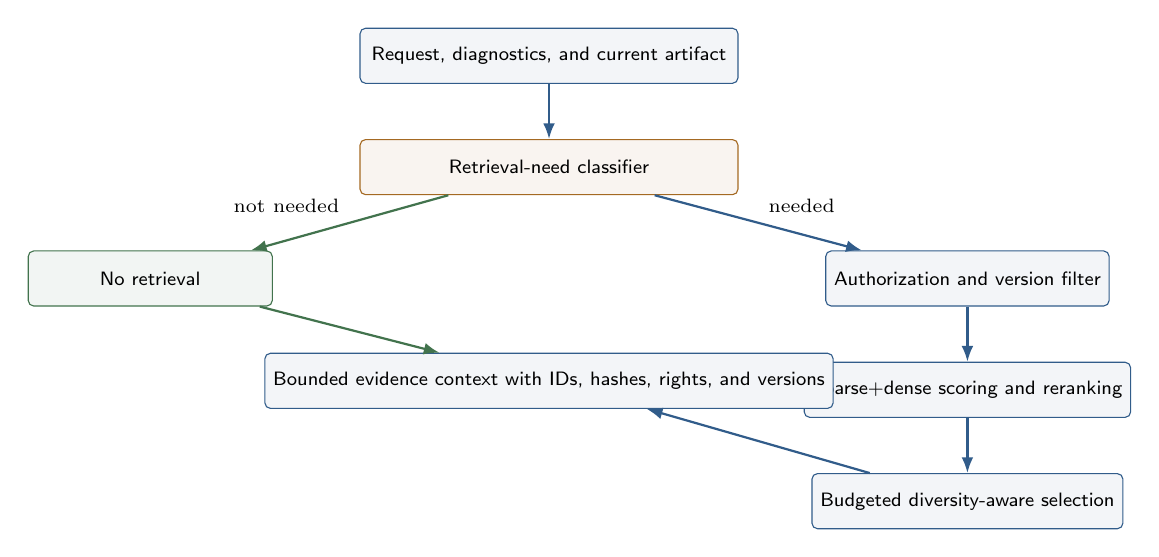
\begin{tikzpicture}[node distance=7mm and 11mm]
  \node[httbox, minimum width=48mm] (request) {Request, diagnostics, and current artifact};
  \node[warnbox, below=of request, minimum width=48mm] (need) {Retrieval-need classifier};
  \node[gatebox, below left=of need] (none) {No retrieval};
  \node[httbox, below right=of need] (filter) {Authorization and version filter};
  \node[httbox, below=of filter] (rank) {Sparse+dense scoring and reranking};
  \node[httbox, below=of rank] (select) {Budgeted diversity-aware selection};
  \node[httbox, below=20mm of need, minimum width=52mm] (context) {Bounded evidence context with IDs, hashes, rights, and versions};
  \draw[httarrow] (request) -- (need);
  \draw[gatearrow] (need) -- node[above left, font=\scriptsize] {not needed} (none);
  \draw[httarrow] (need) -- node[above right, font=\scriptsize] {needed} (filter);
  \draw[httarrow] (filter) -- (rank);
  \draw[httarrow] (rank) -- (select);
  \draw[gatearrow] (none) -- (context);
  \draw[httarrow] (select) -- (context);
\end{tikzpicture}
}
  \caption{\textbf{Selective, version-aware retrieval.}  Authorization and version filtering occurs
  before semantic ranking; selected evidence remains bounded and fully identified.}
  \label{fig:retrieval}
\end{figure}

\subsection{Filtering and hybrid relevance}

For request representation $\vect q$ and evidence chunk $j$, define lexical score $s_j^{\mathrm{lex}}$,
dense similarity $s_j^{\mathrm{dense}}$, cross-encoder score $s_j^{\mathrm{cross}}$, version match
$v_j$, and diagnostic-symbol match $d_j$.  Standardize every continuous feature on development data:
\begin{equation}
  \widetilde s_{jk}=\frac{s_{jk}-\mu_k}{\sigma_k+\epsilon}.
\end{equation}
Only chunks passing rights, principal, tenant, availability-time, product-version, and source-integrity
filters enter the set $\mathcal A(\mathcal R)$.  A relevance utility can then be
\begin{equation}
  u_j=\beta_1\widetilde s_j^{\mathrm{lex}}
      +\beta_2\widetilde s_j^{\mathrm{dense}}
      +\beta_3\widetilde s_j^{\mathrm{cross}}
      +\beta_4v_j+\beta_5d_j.
  \label{eq:retrieval-utility}
\end{equation}
The coefficients are fitted only on retrieval development labels.  Iterative and selective
repository retrieval are supported patterns, not proof for Terminal artifacts
\cite{zhang2023repocoder,wu2024repoformer,zhang2024raft}.

\subsection{Budgeted diversity-aware selection}

Let $c_j$ be the token cost of chunk $j$, including delimiters and citation metadata, and let
$z_j\in\{0,1\}$ indicate selection.  A concrete budgeted objective is
\begin{align}
  \max_{\vect z}\quad
  &\sum_{j\in\mathcal A(\mathcal R)}u_jz_j
  -\lambda_{\mathrm{dup}}\sum_{j<k}\operatorname{sim}(j,k)z_jz_k,\\
  \text{subject to}\quad
  &\sum_j c_jz_j\le B_{\mathrm{evidence}},
  \qquad z_j\in\{0,1\}.
  \label{eq:retrieval-knapsack}
\end{align}
The quadratic penalty discourages redundant chunks.  Greedy marginal-gain selection is an
approximation; the implementation must record the chosen method and deterministic tie breaks.

The complete context budget is
\begin{equation}
  B_{\mathrm{system}}+B_{\mathrm{request}}+B_{\mathrm{evidence}}
  +B_{\mathrm{artifact}}+B_{\mathrm{diagnostic}}+B_{\mathrm{output}}
  +B_{\mathrm{delimiters}}
  \le N_{\max}.
  \label{eq:context-budget}
\end{equation}
Long repositories are never dumped wholesale.  Retrieval recall is evaluated independently from
generation because a generator cannot legitimately compensate for missing authoritative evidence by
inventing an API.

\section{Corpus governance and data-mixture optimization}

Every admitted record binds source identity, license and rights decision, acquisition time, content
hash, product version, knowledge class, deduplication lineage, teacher identity for synthetic data,
tool versions, and validation outcomes.  The partitions are:
\begin{itemize}
  \item \emph{train}: admitted records visible to gradient updates;
  \item \emph{development}: visible tasks for architecture and harness iteration;
  \item \emph{calibration}: threshold fitting, never gradient training;
  \item \emph{sealed}: independently held promotion comparison; and
  \item \emph{future}: SDK- and time-forward cases acquired after the training cutoff.
\end{itemize}
Exact hashes, token MinHash, abstract-syntax-tree fingerprints, dependency graphs, prompts, and
semantic clusters enforce split isolation.  Deduplication is quality control as well as contamination
control \cite{lee2022dedup,lozhkov2024starcoder2}.

Let $k$ index corpus lanes and $\vect\alpha$ be mixture weights on the simplex
$\Delta^{K-1}$.  Mixture selection is a bilevel problem:
\begin{align}
  \vect\theta^*(\vect\alpha)
  &=\argmin_{\vect\theta}
    \sum_{k=1}^{K}\alpha_k\mathcal L_k^{\mathrm{train}}(\vect\theta),\\
  \min_{\vect\alpha\in\Delta^{K-1}}
  &\quad\max_k\widetilde{\mathcal L}_k^{\mathrm{dev}}
        (\vect\theta^*(\vect\alpha)),\\
  \text{subject to}
  &\quad\alpha_k\ge f_k\ge0,qquad \sum_k f_k\le1.
  \label{eq:data-mixture}
\end{align}
Development losses are normalized by a fixed reference so one intrinsically high-entropy lane does
not dominate solely by scale.  Floors $f_k$ protect rare refusal, security, visual-accessibility, and
numeric-edge lanes.  Proxy optimization such as DoReMi is admissible only if it improves sealed
functional slices rather than merely average language-model loss \cite{xie2023doremi}.

\section{Training objectives and curriculum}

\subsection{Domain scaling pilots}

Before a full run, fit domain scaling behavior across multiple model sizes and token budgets.  A
candidate phenomenological form is
\begin{equation}
  \mathcal L(P,D)=\mathcal L_\infty+aP^{-\alpha}+bD^{-\beta},
  \qquad a,b,\alpha,\beta>0,
  \label{eq:scaling-law}
\end{equation}
where $D$ is admitted training tokens.  Four parameter sizes at one token budget cannot identify
both exponents; each size needs multiple budgets or a preregistered constrained fit.  Functional
metrics and contamination checks remain primary because perplexity scaling does not establish
artifact correctness.

\subsection{Masked, task-balanced next-token prediction}

Let a serialized example contain target tokens $z_1,\ldots,z_T$, immutable context $c$, and
nonnegative weights $w_t$.  The normalized next-token loss is
\begin{equation}
  \mathcal L_{\mathrm{NTP}}
  =-\frac{\sum_{t=1}^{T}w_t
      \log p_{\vect\theta}(z_t\mid z_{<t},c)}
     {\sum_{t=1}^{T}w_t},
  \qquad \sum_tw_t>0.
  \label{eq:ntp}
\end{equation}
Prompt, padding, retrieved evidence, tool output, and rejected-output regions receive $w_t=0$.
Approved artifacts and concise visible planning fields receive lane- and region-balanced weights.
The denominator prevents long examples from dominating solely by token count.

For task lanes $k$ sampled with target weights $\pi_k$, one implementation first computes a
token-normalized example loss and then averages per task:
\begin{equation}
  \mathcal L_{\mathrm{balanced}}
  =\sum_k\pi_k\frac{1}{|\mathcal B_k|}
     \sum_{e\in\mathcal B_k}\mathcal L_{\mathrm{NTP}}^{(e)}.
  \label{eq:task-balanced-loss}
\end{equation}

\subsection{Verified supervised fine-tuning and distillation}

For artifact regions $r\in\mathcal R_{\mathrm{region}}$, define each
$\mathcal L_r$ as a token-normalized NLL.  The supervised objective is
\begin{equation}
  \mathcal L_{\mathrm{SFT}}=\sum_r\lambda_r\mathcal L_r,
  \qquad \lambda_r\ge0,quad\sum_r\lambda_r=1.
  \label{eq:sft}
\end{equation}
Regions include artifact text, bounded plan, evidence use, refusal/abstention, and diagnostic repair.
Teacher rationales are not treated as executable evidence and private hidden chain-of-thought is not
retained.

When teacher and student logits are available over the same allowed vocabulary, temperature-$T_d$
distillation uses
\begin{equation}
  \mathcal L_{\mathrm{KD}}
  =T_d^2\sum_t
  \KL\!\left(
    p_{\mathrm{teacher}}^{(T_d)}(\cdot\mid z_{<t},c)
    \;\middle\|\;
    p_{\vect\theta}^{(T_d)}(\cdot\mid z_{<t},c)
  \right).
  \label{eq:distillation}
\end{equation}
The $T_d^2$ factor compensates the gradient shrinkage introduced by softening.  Every distilled
artifact must still pass stronger deterministic checks than those visible to the teacher
\cite{hsieh2023distill}.

\subsection{Preference optimization}

Preference data is permitted only when both candidates already pass identical hard gates and differ
in readability, maintainability, minimality, idiom, or visual clarity.  For prompt $x$, preferred
$y_w$, rejected $y_l$, policy $\pi_{\vect\theta}$, fixed reference $\pi_{\mathrm{ref}}$, and
temperature $\beta>0$, direct preference optimization uses
\begin{align}
  \Delta_{\vect\theta}(x,y_w,y_l)
  &=\log\frac{\pi_{\vect\theta}(y_w\mid x)}{\pi_{\mathrm{ref}}(y_w\mid x)}
   -\log\frac{\pi_{\vect\theta}(y_l\mid x)}{\pi_{\mathrm{ref}}(y_l\mid x)},\\
  \mathcal L_{\mathrm{DPO}}
  &=-\E_{(x,y_w,y_l)}\left[
    \log\sigmoid\!\left(\beta\Delta_{\vect\theta}(x,y_w,y_l)\right)
  \right].
  \label{eq:dpo}
\end{align}
Sequence log probabilities are sums of token log probabilities under the same grammar support.
Preference optimization cannot promote an incorrect candidate over a correct one
\cite{rafailov2023dpo}.

\subsection{Reinforcement learning with verifiable rewards}

An additive reward can accidentally allow soft quality to rescue a schema or policy failure.  HTT
therefore defines a hard indicator $H(y,x)$ as in \cref{eq:hard-feasible} and bounded utility
$U(y,x)\in[0,1]$.  A scalar representation that preserves the lexicographic order is
\begin{equation}
  R(y,x)=
  \begin{cases}
    -1-C_{\mathrm{fail}}(y,x), & H(y,x)=0,\\
    1+U(y,x)-\lambda_c C_{\mathrm{cost}}(y,x), & H(y,x)=1,
  \end{cases}
  \label{eq:hard-reward}
\end{equation}
where $C_{\mathrm{fail}}\ge0$ and the accepted-branch cost is bounded so
$\lambda_cC_{\mathrm{cost}}<1$.  Every feasible artifact then outranks every infeasible artifact.
Backtest profit is excluded because it is unstable, exploitable, and regime dependent.

For a group of $G_{\mathrm{group}}$ candidates with rewards $R_i$, define sample mean and stabilized
advantage
\begin{align}
  \bar R&=\frac{1}{G_{\mathrm{group}}}\sum_iR_i,\\
  s_R&=\sqrt{\frac{1}{G_{\mathrm{group}}-1}\sum_i(R_i-\bar R)^2},\\
  A_i&=\frac{R_i-\bar R}{s_R+\epsilon_R}.
  \label{eq:group-advantage}
\end{align}
For token ratio
$\rho_{it}=\pi_{\vect\theta}(z_{it}\mid z_{i,<t},x)/
\pi_{\mathrm{old}}(z_{it}\mid z_{i,<t},x)$, a clipped group-relative objective is
\begin{equation}
  \mathcal L_{\mathrm{GRPO}}
  =-\E_{i,t}\left[
     \min\left(\rho_{it}A_i,
       \clip(\rho_{it},1-\epsilon_c,1+\epsilon_c)A_i\right)
   -\beta_{\mathrm{KL}}\KL(\pi_{\vect\theta}\|\pi_{\mathrm{ref}})
  \right].
  \label{eq:grpo}
\end{equation}
If the group variance is zero, advantages are set to zero rather than amplified by a tiny denominator.
For leave-one-out baselines,
\begin{equation}
  b_i=\frac{1}{G_{\mathrm{group}}-1}\sum_{j\ne i}R_j,
  \qquad A_i=R_i-b_i.
  \label{eq:rloo}
\end{equation}
\abbr{GRPO}, \abbr{RLOO}, and ordinary supervised learning are controlled alternatives, not assumed
winners \cite{ahmadian2024rloo,shao2024deepseekmath}.

\subsection{Multi-token prediction}

For $H$ auxiliary future-token heads, bounded indices, and nonnegative weights $\lambda_j$,
\begin{equation}
  \mathcal L_{\mathrm{MTP}}
  =-\sum_{j=1}^{H}\frac{\lambda_j}{T-j}
    \sum_{t=1}^{T-j}
    \log p_{\vect\theta,j}(z_{t+j}\mid z_{\le t},c).
  \label{eq:mtp}
\end{equation}
Auxiliary-head parameters, training FLOPs, and removal or reuse at inference must be reported.
Published gains are scale dependent; HTT retains next-token prediction unless 450M- and 900M-parameter
pilots show a functional improvement without reducing trunk depth \cite{gloeckle2024mtp}.

\section{Grammar-constrained generation and candidate selection}

\subsection{Normalized grammar-masked distribution}

At decoding step $t$, let logits be $z_{t,v}$ and let the deterministic incremental parser expose
allowed token set $\mathcal A_t$.  The constrained distribution is
\begin{equation}
  p_{\mathrm{mask}}(v\mid y_{<t},x)
  =\frac{\exp(z_{t,v})\1[v\in\mathcal A_t]}
         {\sum_{u\in\mathcal A_t}\exp(z_{t,u})}.
  \label{eq:grammar-mask}
\end{equation}
Every disallowed token has exactly zero probability, and the denominator renormalizes over valid
continuations.  If $\mathcal A_t=\varnothing$, generation terminates as a parser failure rather than
falling back to an unconstrained vocabulary.  Grammar masking guarantees syntax only; types,
capabilities, semantics, and behavior remain external gates \cite{ugare2024syncode}.

\subsection{Hard-feasible candidate selection}

For candidate $i$, define length-normalized model log likelihood
\begin{equation}
  \bar\ell_i=\frac{1}{|y_i|}\sum_{t=1}^{|y_i|}
  \log p_{\vect\theta}(y_{it}\mid y_{i,<t},x).
  \label{eq:length-normalized-logp}
\end{equation}
Let $\vect z_i$ contain $\bar\ell_i$, compiler diagnostics, test coverage, mutation score, visual
metrics, retrieval support, cost, and a learned verifier output.  Continuous features are standardized
with calibration-set means and scales.  A linear reference selector is
\begin{equation}
  s_i=\vect w^\top\widetilde{\vect z}_i.
  \label{eq:candidate-score}
\end{equation}
Selection occurs only inside the hard-feasible set:
\begin{equation}
  \widehat i_j=\argmax_{i\in\mathcal F_j}s_{ji}.
  \label{eq:feasible-argmax}
\end{equation}
If the set is empty, the request abstains or enters bounded repair.  Execution-aware learned
verification can improve ranking in prior code-generation settings, but HTT requires an independently
trained verifier, near-miss mutants, calibration, and sealed tests \cite{ni2023lever,cobbe2021verifiers}.

\subsection{Calibration after selection}

Selecting the maximum of $K_{\mathrm{cand}}$ candidates changes the score distribution.  Calibration
therefore occurs at request level \emph{after} \cref{eq:feasible-argmax}, separately for each serving
candidate budget and quantization profile.  Let $q_j\in[0,1]$ be calibrated probability that selected
artifact $\widehat i_j$ passes the sealed-equivalent outcome, and let $Y_j\in\{0,1\}$ be that outcome.
For threshold $\tau$,
\begin{align}
  \mathcal I_\tau&=\{j:q_j\ge\tau\},\\
  \widehat{\Coverage}(\tau)
  &=\frac{|\mathcal I_\tau|}{N_{\mathrm{eval}}},\\
  \widehat{\Risk}(\tau)
  &=\frac{\sum_{j\in\mathcal I_\tau}(1-Y_j)}{|\mathcal I_\tau|},
  \qquad |\mathcal I_\tau|>0.
  \label{eq:risk-coverage}
\end{align}
Risk is undefined at zero coverage.  The threshold is chosen on calibration data using an upper
confidence bound, not the point estimate alone.  If $e_\tau$ failures occur among $n_\tau$ accepted
requests, a one-sided Clopper--Pearson upper bound is
\begin{equation}
  U_\alpha(e_\tau,n_\tau)
  =F^{-1}_{\mathrm{Beta}}(1-\alpha;e_\tau+1,n_\tau-e_\tau),
  \label{eq:cp-upper}
\end{equation}
with the conventional boundary case for $e_\tau=n_\tau$.  Choose the lowest threshold satisfying
$U_\alpha\le r_{\max}$ and a minimum coverage constraint.  This protects against accepting a tiny,
apparently perfect sample.

Calibration diagnostics include Brier score
\begin{equation}
  \operatorname{Brier}=\frac{1}{N_{\mathrm{eval}}}
  \sum_{j=1}^{N_{\mathrm{eval}}}(q_j-Y_j)^2,
  \label{eq:brier}
\end{equation}
negative log likelihood
\begin{equation}
  \NLL=-\frac{1}{N_{\mathrm{eval}}}\sum_j
  \left[Y_j\log q_j+(1-Y_j)\log(1-q_j)\right],
  \label{eq:calibration-nll}
\end{equation}
and bin-based expected calibration error
\begin{equation}
  \ECE=\sum_{b=1}^{B_{\mathrm{bin}}}
  \frac{|I_b|}{N_{\mathrm{eval}}}
  \left|\frac{1}{|I_b|}\sum_{j\in I_b}Y_j
       -\frac{1}{|I_b|}\sum_{j\in I_b}q_j\right|.
  \label{eq:ece}
\end{equation}
Because \abbr{ECE} depends on bins and can hide local error, reliability plots, Brier score, NLL, and
risk--coverage curves are all reported \cite{kadavath2022calibration}.

\section{Verification and evaluation architecture}

\begin{figure}[t]
  \centering
  \resizebox{\linewidth}{!}{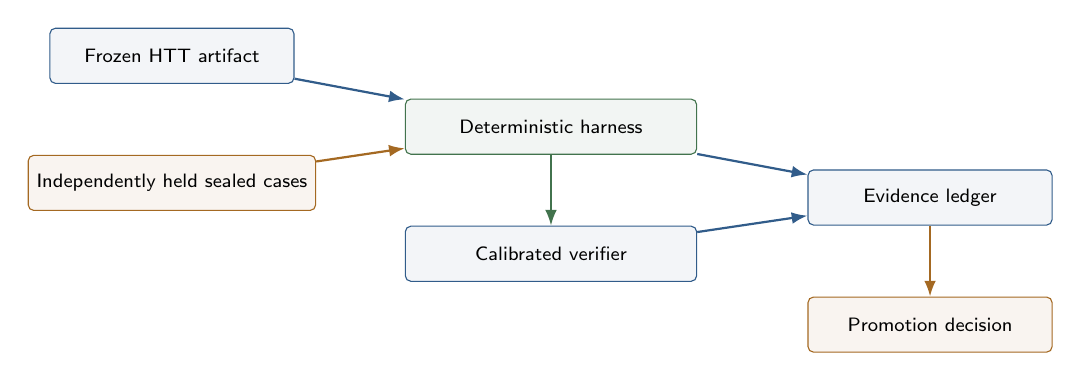
\begin{tikzpicture}[node distance=9mm and 14mm]
  \node[httbox] (model) {Frozen HTT artifact};
  \node[warnbox, below=of model] (cases) {Independently held sealed cases};
  \node[gatebox, right=of model, yshift=-9mm, minimum width=37mm] (harness) {Deterministic harness};
  \node[httbox, below=of harness, minimum width=37mm] (verifier) {Calibrated verifier};
  \node[httbox, right=of harness, yshift=-9mm] (ledger) {Evidence ledger};
  \node[warnbox, below=of ledger] (decision) {Promotion decision};
  \draw[httarrow] (model) -- (harness);
  \draw[warnarrow] (cases) -- (harness);
  \draw[gatearrow] (harness) -- (verifier);
  \draw[httarrow] (harness) -- (ledger);
  \draw[httarrow] (verifier) -- (ledger);
  \draw[warnarrow] (ledger) -- (decision);
\end{tikzpicture}
}
  \caption{\textbf{Independent evidence path.}  The model, trainer, and coordinator cannot write
  sealed labels or modify promotion policy.  Evidence informs a later human decision.}
  \label{fig:evaluation}
\end{figure}

\subsection{Hard strategy and visualizer gates}

Every strategy candidate must satisfy closed schema, exact-hash recomputation, parse and compile
against the pinned SDK, namespace/type/member policy, isolated resource limits, deterministic tests,
edge cases, metamorphic tests, mutation tests, and prohibited-capability scans.  Every visualizer
candidate must satisfy schema, allowlisted data sources and transforms, bounded geometry and update
cost, deterministic rendering, screenshot/geometry comparison, accessibility, interaction replay,
fallback behavior, and prohibited-capability scans.  A learned verifier is supplementary evidence,
not a substitute for these checks.

\subsection{Primary request-level metrics}

Let $A_j\in\{0,1\}$ indicate that request $j$ is accepted after selection and calibration, and let
$Y_j\in\{0,1\}$ denote functional correctness of its selected artifact.  Three quantities must be
reported together:
\begin{align}
  \widehat{\mathrm{coverage}}
  &=\frac{1}{N_{\mathrm{eval}}}\sum_jA_j,\\
  \widehat{\mathrm{selective\ accuracy}}
  &=\frac{\sum_jA_jY_j}{\sum_jA_j},
  \quad\sum_jA_j>0,\\
  \widehat{\mathrm{accepted\ yield}}
  &=\frac{1}{N_{\mathrm{eval}}}\sum_jA_jY_j.
  \label{eq:accepted-metrics}
\end{align}
The third equals coverage times selective accuracy.  Reporting selective accuracy without coverage
can reward a system that abstains on almost everything; reporting yield without selective risk can
hide unsafe acceptance.

Compile-at-one is the fraction whose first generated candidate compiles without repair.  Sealed
functional pass-at-one is the fraction whose final deterministic-selection output passes the complete
hidden suite under a fixed attempt budget.  Candidate count, tool-call budget, context, evidence, and
selection policy are part of the evaluated system and cannot differ across models without being
reported.

\subsection{Pass-at-$k$ derivation}

Suppose $n$ sampled candidates contain $c$ correct candidates and we choose $k\le n$ without
replacement.  There are $\binom nk$ equally sized subsets.  The subsets containing no correct
candidate choose all $k$ elements from the $n-c$ incorrect candidates, so
\begin{equation}
  \Prob(\text{zero correct in }k)=\frac{\binom{n-c}{k}}{\binom nk}.
\end{equation}
Taking the complement gives the standard estimator
\begin{equation}
  \widehat{\mathrm{pass@}k}
  =1-\frac{\binom{n-c}{k}}{\binom nk}.
  \label{eq:pass-at-k}
\end{equation}
It assumes exchangeable samples from a fixed generation policy.  HTT's primary metric remains
pass-at-one after a fixed deterministic selector; pass-at-$k$ is diagnostic because larger sampling
budgets spend more compute \cite{chen2021humaneval}.

\subsection{Perplexity and tokenizer comparability}

For normalized natural-log NLL $\overline{\mathcal L}$,
\begin{equation}
  \operatorname{PPL}=\exp(\overline{\mathcal L}).
  \label{eq:perplexity}
\end{equation}
Per-token perplexity is not directly comparable across tokenizers because the atomic events differ.
Tokenizer studies therefore also report NLL per byte or character and functional artifact metrics.

\subsection{Paired significance and power}

For two systems $A$ and $B$ evaluated on identical requests, let $n_{10}$ count cases where only
$A$ succeeds and $n_{01}$ cases where only $B$ succeeds.  The estimated paired difference is
\begin{equation}
  \widehat\Delta=\frac{n_{10}-n_{01}}{N_{\mathrm{eval}}}.
  \label{eq:paired-delta}
\end{equation}
Under the null that discordant outcomes are equally likely, exact McNemar testing treats
$n_{10}\mid(n_{10}+n_{01})$ as $\operatorname{Binomial}(n_{10}+n_{01},1/2)$.  When discordant counts
are sufficiently large, the continuity-corrected approximation is
\begin{equation}
  \chi^2=\frac{(|n_{10}-n_{01}|-1)^2}{n_{10}+n_{01}}.
  \label{eq:mcnemar}
\end{equation}

Power depends on discordance, not only total accuracy.  Let
$p_{10}=\Prob(A=1,B=0)$, $p_{01}=\Prob(A=0,B=1)$, and
$\Delta_*=p_{10}-p_{01}$ be the smallest meaningful paired improvement.  A normal-approximation
planning equation is
\begin{equation}
  N_{\mathrm{eval}}
  \approx
  \frac{(z_{1-\alpha/2}+z_{1-\beta})^2
  \left(p_{10}+p_{01}-\Delta_*^2\right)}{\Delta_*^2}.
  \label{eq:paired-power}
\end{equation}
The preregistration must supply plausible discordance from pilot data, desired power $1-\beta$, and
multiplicity correction.  ``At least three seeds'' does not create a reliable seed-level confidence
interval; examples are sampled across sufficient independent training runs or modeled hierarchically.

Repository families, synthetic lineages, and near-duplicate prompts violate request-level
independence.  Paired bootstrap resampling therefore operates at the highest independent
repository/lineage cluster.  Architecture comparisons use Holm correction or reserve an untouched
confirmation set.  Efficiency comparisons require identical hardware, precision, runtime, batch
policy, context, output length, and thermal state.

\subsection{Contamination and future evaluation}

Training, teacher, retrieval, and generated corpora are compared with evaluation material using exact
hashes, token similarity, AST and graph fingerprints, prompt lineage, and semantic clusters.  A
rolling future suite contains SDK and schema tasks acquired after the training cutoff.  Public rolling
suites eventually become trainable and cannot remain sealed forever; LiveCodeBench motivates the
post-cutoff pattern but does not replace private Terminal cases \cite{jain2024livecodebench}.

\section{Inference and serving mathematics}

\subsection{Artifact identity and request path}

A served artifact identity binds weights, tokenizer, active task lane, quantization, runtime, kernels,
context policy, retrieval pack, grammar, verifier, calibration map, and threshold.  Any change creates
a new evaluated artifact.  The request path is
\begin{equation}
  \begin{aligned}
    \text{authenticate}&\rightarrow\text{authorize}\rightarrow\text{bind purpose}
      \rightarrow\text{retrieve}\rightarrow\text{generate}\rightarrow\text{gate}\\
    &\rightarrow\text{select}\rightarrow\text{calibrate}\rightarrow\text{inert artifact}.
  \end{aligned}
\end{equation}

\subsection{Quantization model and non-inferiority}

For affine $b$-bit quantization with scale $s>0$, zero point $z$, integer range
$[q_{\min},q_{\max}]$, and weight $w$,
\begin{align}
  q(w)&=\clip\!\left(\operatorname{round}(w/s)+z,q_{\min},q_{\max}\right),\\
  \widehat w&=s(q(w)-z).
  \label{eq:affine-quant}
\end{align}
When no clipping occurs, rounding gives $|w-\widehat w|\le s/2$.  Network error can still compound
through layers and grammar-boundary logits, so a per-weight bound does not establish artifact parity.
Weight-only INT8, weight-only W4A16 AWQ/GPTQ, and W8A8 profiles are separate artifacts
\cite{frantar2023gptq,lin2024awq,xiao2023smoothquant}.

For paired functional outcomes, let $\Delta_q=p_{\mathrm{quant}}-p_{\mathrm{BF16}}$ and choose a
non-inferiority margin $\delta>0$.  Quantization passes only if the one-sided lower confidence bound
satisfies
\begin{equation}
  \operatorname{LCB}_{1-\alpha}(\Delta_q)>-\delta,
  \label{eq:quant-ni}
\end{equation}
while every hard gate, calibration ceiling, coverage floor, and slice-specific safety metric also
passes.  Average non-inferiority cannot compensate for a prohibited-capability regression.

\subsection{Continuous batching and cache isolation}

Batching is allowed only among compatible artifact identities and privacy domains.  Prefix reuse
requires identical tenant authorization, evidence hash, task lane, model, grammar, and policy.  User
or private-evidence prefixes are never shared across unauthorized principals.  Released cache pages
are zeroized according to the serving threat model.  The capacity constraint for live sequences $j$
is
\begin{equation}
  \sum_j M_{\mathrm{KV,hybrid}}(B_j,N_j)
  +M_{\mathrm{weights}}+M_{\mathrm{workspace}}+M_{\mathrm{activations}}
  \le M_{\mathrm{device,reserved}},
  \label{eq:serving-memory}
\end{equation}
with an explicit safety reserve rather than optimistic use of all device memory.

\subsection{Speculative decoding}

Let draft distribution $q(x)$ and target distribution $p(x)$ have identical grammar support.  A draft
token $x\sim q$ is accepted with
\begin{equation}
  a(x)=\min\!\left(1,\frac{p(x)}{q(x)}\right).
  \label{eq:spec-accept}
\end{equation}
On rejection, sample from residual distribution
\begin{equation}
  r(x)=\frac{(p(x)-q(x))_+}{\sum_u(p(u)-q(u))_+}.
  \label{eq:spec-residual}
\end{equation}
These rules preserve the target distribution; greedy acceptance does not.  Speculation is optional
and must retain identical grammar masks, deterministic tool boundaries, and artifact parity
\cite{leviathan2023speculative}.

\subsection{Operational gates, not performance claims}

The initial qualification records p50/p95 time to first token, tokens per second, tool latency,
request latency, peak device and host memory, power, and energy per accepted artifact at 8K, 16K, and
32K contexts.  Gates include no out-of-memory at admitted concurrency, no hard-gate regression,
request-level calibration within its ceiling, deterministic replay, and clean rollback.  No number in
this protocol claims that those gates have been met.

\section{Ablation design and parameter matching}

An ablation changes one hypothesis while holding data order, token budget, optimizer, evaluation,
context, candidate/tool budget, and hardware constant.  Raw-shape comparisons and parameter-matched
comparisons answer different questions and both are reported.

Changing $h_{\mathrm{kv}}$ from 4 to 16 at fixed $d,d_h$ adds per block
\begin{align}
  \Delta P_{\mathrm{MHA,block}}
  &=2d(16-4)d_h\\
  &=2(2{,}048)(12)(128)=6{,}291{,}456,
\end{align}
or
\begin{equation}
  \Delta P_{\mathrm{MHA,total}}=32(6{,}291{,}456)=201{,}326{,}592.
  \label{eq:mha-extra}
\end{equation}
Reducing SwiGLU width from 5,632 to 4,608 removes exactly
$3d(5{,}632-4{,}608)=6{,}291{,}456$ parameters per block, giving a parameter-matched MHA control.
The raw control measures the direct engineering replacement; the compensated control separates head
sharing from total capacity.

\begin{longtable}{@{}L{0.12\linewidth}L{0.27\linewidth}L{0.24\linewidth}L{0.27\linewidth}@{}}
\caption{Mandatory architecture ablations.}\label{tab:ablations}\\
\toprule ID & Change & Control & Primary decision signal \\
\midrule
\endfirsthead
\toprule ID & Change & Control & Primary decision signal \\
\midrule
\endhead
A1 & all-global attention & 3:1 hybrid & functional accuracy versus memory/latency \\
A2 & 5:1 local/global & 3:1 hybrid & efficiency without long-context regression \\
A3 & 2K and 8K local windows & 4K & context-slice correctness and cache \\
A4 & 1, 2, 8, 16 KV heads & 4 & quality, cache, and compensated capacity \\
A5 & remove task lanes & rank-64 lanes & interference by artifact family \\
A6 & rank 32 and 128 & rank 64 & accuracy per active parameter \\
A7 & remove parser embedding & optional table & value beyond mandatory grammar mask \\
A8 & 16K, 32K, 48K vocabulary & 32K & tokens, exact copy, quality, embedding size \\
A9 & 24 and 36 blocks & 32 & depth at matched active parameters \\
A10 & QK-Norm off & QK-Norm on & stability and functional quality \\
\bottomrule
\end{longtable}

Deferred challengers include mixture of experts, dynamic depth, state-space hybrids, byte-latent
tokenization, ternary weights, and native vision.  They enter only after the dense reference is
reproducible \cite{raposo2024mod,dao2024mamba2,pagnoni2024blt,ma2024bitnet}.

\section{Security, privacy, and failure analysis}

\begin{longtable}{L{0.24\linewidth}L{0.28\linewidth}L{0.38\linewidth}}
\caption{Principal failure modes and controls.}\label{tab:failures}\\
\toprule Failure & Why it matters & Required control \\
\midrule
\endfirsthead
\toprule Failure & Why it matters & Required control \\
\midrule
Hallucinated API & compiles against no real SDK & versioned retrieval, exact compile, abstention \\
Semantically wrong strategy & syntax is insufficient & properties, metamorphic and mutation tests \\
Prompt injection in evidence & retrieved text may claim authority & provenance, instruction/data separation, quarantine \\
Prohibited capability & generated source exceeds scope & closed schemas, compiler/IL scan, sandbox \\
Authority-field fabrication & model attempts self-approval & coordinator recomputes and rejects fields \\
Verifier reward hacking & score exceeds real quality & independent hidden tests, near-miss mutants, rotation \\
Cross-request leakage & private context reaches another user & cache isolation, zeroization, canaries \\
Training contamination & sealed answers become memorized & lineage graph, time split, independent custody \\
Quantization drift & boundary logits or behavior change & paired non-inferiority and hard-gate parity \\
Distribution shift & SDK or conventions change & future suite, retrieval versioning, rollback \\
\bottomrule
\end{longtable}

Privacy testing uses approved synthetic canaries for exact and approximate extraction, membership
inference, cross-request leakage, prefix-cache isolation, log redaction, retention, deletion, teacher
exposure, and quantized-artifact parity.  Real secrets are never used as probes.  The model card must
state that the system is purpose-limited, cannot predict markets, has no trading authority, may
abstain, requires deterministic validation, and has not been shown correct until sealed evidence
exists.

\section{Implementation roadmap and decision gates}

\begin{description}[style=nextline,leftmargin=0pt]
\item[Gate 0 --- protocol review.] Review purpose, artifact boundaries, mathematical assumptions,
corpus rights, architecture candidates, target hardware, evaluation ownership, and budget.
\item[Gate 1 --- data and tokenizer readiness.] Require an audited corpus manifest, split-isolation
report, tokenizer study, executable harnesses, and preregistered metrics.
\item[Gate 2 --- small-pilot selection.] Train at least three parameter-matched candidates at each of
several sizes and token budgets; select using functional and efficiency evidence, not perplexity alone.
\item[Gate 3 --- scaling authorization.] Fit scaling curves, profile achieved utilization, rehearse
checkpoint recovery, and approve the full-run budget separately.
\item[Gate 4 --- frozen-model evaluation.] Freeze weights, tokenizer, runtime, quantization, retrieval,
grammar, verifier, calibration map, and thresholds before an independent operator unseals results.
\item[Gate 5 --- promotion and shadow serving.] Require signed evidence, no hard-gate regression,
accepted risk, rollback, startup attestation, and inert shadow artifacts.
\item[Gate 6 --- constrained rollout.] Begin with low-risk mock/research use, strict capacity, logging,
and human review; expand only from monitored evidence.
\end{description}

\section{Limitations and falsifiability}

The paper describes an architecture and protocol, not a trained model.  A narrow 1.5B model may
underfit compositional language, overfit templates, or require more clean tokens than the rights-approved
domain corpus can supply.  Scratch training avoids inherited data uncertainty but may be worse than
continued pretraining from an eligible small code model; both must be compared under the same
retrieval, tools, and evaluation \cite{pinnaparaju2024stablecode}.  Long mathematical derivations do
not establish kernel performance, generalization, or safety.  Grammar masks establish syntax, not
meaning.  Deterministic tests are only as strong as their coverage.  Verifiers can be miscalibrated or
reward-hacked.  Human approval can fail operationally.

The proposal is rejected or revised if a simpler parameter-matched baseline wins sealed functional
pass-at-one, if the narrow corpus cannot support future-version generalization, if quantization breaks
hard gates, if request-level risk cannot be bounded at useful coverage, or if latency/memory targets
cannot be met on intended hardware.  Architectural novelty is not a promotion criterion.

\section{Conclusion}

HTT-1.5B-r0 is a conservative transformer embedded in an aggressive verification boundary.  Stable
skills enter weights; mutable private facts enter signed retrieval; syntax is restricted by a parser;
semantics are judged by compilers, renderers, and tests; uncertainty is handled after candidate
selection; and release remains external.  The proposed dimensions imply a 1.523B core stored model,
a 1.524B parser-enabled model, and a 0.6875 GiB batch-one BF16 KV cache at 32K under the stated hybrid
schedule.  The derivations make those claims auditable and distinguish causal prefill from decode,
weight memory from training state, and score-position savings from total runtime.

The next research deliverables are a governed corpus manifest, tokenizer report, executable sealed
harness, small-model scaling and ablation report, and calibrated request-level selector.  Only those
experiments can determine whether the architecture is accurate, fast, parameter-efficient, and safely
narrow enough for Terminal strategy and visualizer authoring.

\appendix

\section{Additional derivations and dimensional checks}

\subsection{Leading-order parameter expression}

Ignoring small normalization, identity, adapter, and parser terms, a tied-embedding GQA/SwiGLU model
has
\begin{equation}
  P_{\mathrm{lead}}
  =|\mathcal V|d+n_{\mathrm{layer}}
    \left[2d^2+2dh_{\mathrm{kv}}d_h+3dd_{\mathrm{ff}}\right].
  \label{eq:leading-param}
\end{equation}
If $h_qd_h=d$ and $d_{\mathrm{ff}}\approx8d/3$,
\begin{equation}
  P_{\mathrm{lead}}
  \approx|\mathcal V|d+n_{\mathrm{layer}}d^2
  \left(10+2\frac{h_{\mathrm{kv}}}{h_q}\right).
  \label{eq:leading-param-ratio}
\end{equation}
MHA has $h_{\mathrm{kv}}/h_q=1$ and coefficient 12; 4:1 GQA has ratio $1/4$ and
coefficient 10.5.  This expression is useful for matched-shape reasoning but is not the executable
parameter total in \cref{tab:parameter-ledger}.

\subsection{Units audit}

In \cref{eq:weight-memory}, parameters multiplied by bytes per parameter yield bytes.  In
\cref{eq:kv-general}, the factors are key/value copies, batch, layers, tokens, heads, elements per
head, and bytes per element, again yielding bytes.  In \cref{eq:6pt}, parameters and tokens are
dimensionless counts and the coefficient carries approximate floating-point operations per
parameter-token.  In \cref{eq:retrieval-knapsack}, every utility term is standardized and therefore
dimensionless while the constraint is measured in tokens.  These checks prevent adding quantities
with incompatible scales.

\section{Proposed visualizer-IR validation rules}

The proposed visualizer artifact obeys the following minimum rules:
\begin{enumerate}
  \item \code{schemaVersion} is exactly \code{hyperion-terminal-visualizer/v1}.
  \item Every pane references a declared, allowlisted data source.
  \item Every signal is an allowlisted transform with finite cost and explicit null behavior.
  \item Every interaction has bounded, deterministic behavior and no arbitrary callback.
  \item Rendering rejects zero-area panes, duplicate identifiers, invalid scales, and unsupported
        update rates.
  \item Style values come from bounded enums/ranges or approved theme tokens.
  \item Network, filesystem, process, reflection, package, native-code, broker, and credential
        concepts are unrepresentable.
  \item The compiler emits only an approved renderer and records the source schema, compiler version,
        and output hash.
  \item Screenshot, geometry, interaction, accessibility, and performance checks must pass before
        human review.
\end{enumerate}

\section{Minimum sealed-suite composition}

The final model-selection set includes, without reusing calibration cases:
\begin{itemize}
  \item held-out strategy DSL, C\#, numeric, and state-machine problems;
  \item held-out visualizer grammar and accessibility problems;
  \item compile and runtime failures requiring exact repair;
  \item current, stale, missing, contradictory, and adversarial evidence;
  \item prohibited capability and injection tests;
  \item 8K, 16K, 32K, and short-context regression slices;
  \item byte, Unicode, numeric, locale, and unusual-identifier cases;
  \item future SDK/schema tasks acquired after corpus closure; and
  \item enough independent repository/lineage clusters to meet the preregistered paired-power plan.
\end{itemize}

\section{Reproducibility checklist}

\begin{itemize}
  \item Freeze source revision, container/compiler, tokenizer, data manifest, data order, optimizer,
        scheduler, random-number states, kernels, and hardware topology.
  \item Record executable parameter counts rather than relying only on analytic estimates.
  \item Record per-slice losses and functional metrics at every checkpoint.
  \item Keep development, calibration, sealed, and future custody separate.
  \item Bind every result to candidate count, tool budget, context, retrieval pack, and verifier.
  \item Publish negative and null ablations, not only the winning configuration.
  \item Rebuild the paper from this LaTeX source and retain compiler logs with the submission bundle.
\end{itemize}

\begin{thebibliography}{99}
\small

\bibitem{vaswani2017attention}
A.~Vaswani et al. ``Attention Is All You Need.'' \emph{NeurIPS}, 2017.
\url{https://arxiv.org/abs/1706.03762}.

\bibitem{zhang2019rmsnorm}
B.~Zhang and R.~Sennrich. ``Root Mean Square Layer Normalization.'' \emph{NeurIPS}, 2019.
\url{https://arxiv.org/abs/1910.07467}.

\bibitem{shazeer2020glu}
N.~Shazeer. ``GLU Variants Improve Transformer.'' 2020.
\url{https://arxiv.org/abs/2002.05202}.

\bibitem{su2021roformer}
J.~Su et al. ``RoFormer: Enhanced Transformer with Rotary Position Embedding.'' 2021.
\url{https://arxiv.org/abs/2104.09864}.

\bibitem{ainslie2023gqa}
J.~Ainslie et al. ``GQA: Training Generalized Multi-Query Transformer Models from Multi-Head
Checkpoints.'' \emph{EMNLP}, 2023. \url{https://arxiv.org/abs/2305.13245}.

\bibitem{dao2022flashattention}
T.~Dao et al. ``FlashAttention: Fast and Memory-Efficient Exact Attention with IO-Awareness.''
\emph{NeurIPS}, 2022. \url{https://arxiv.org/abs/2205.14135}.

\bibitem{dao2023flashattention2}
T.~Dao. ``FlashAttention-2: Faster Attention with Better Parallelism and Work Partitioning.'' 2023.
\url{https://arxiv.org/abs/2307.08691}.

\bibitem{jiang2023mistral}
A.~Q.~Jiang et al. ``Mistral 7B.'' 2023. \url{https://arxiv.org/abs/2310.06825}.

\bibitem{raposo2024mod}
D.~Raposo et al. ``Mixture-of-Depths: Dynamically Allocating Compute in Transformer-Based Language
Models.'' 2024. \url{https://arxiv.org/abs/2404.02258}.

\bibitem{gloeckle2024mtp}
F.~Gloeckle et al. ``Better \& Faster Large Language Models via Multi-token Prediction.'' 2024.
\url{https://arxiv.org/abs/2404.19737}.

\bibitem{hui2024qwen25}
B.~Hui et al. ``Qwen2.5-Coder Technical Report.'' 2024.
\url{https://arxiv.org/abs/2409.12186}.

\bibitem{guo2024deepseekcoder}
D.~Guo et al. ``DeepSeek-Coder: When the Large Language Model Meets Programming---The Rise of Code
Intelligence.'' 2024. \url{https://arxiv.org/abs/2401.14196}.

\bibitem{lewis2020rag}
P.~Lewis et al. ``Retrieval-Augmented Generation for Knowledge-Intensive NLP Tasks.''
\emph{NeurIPS}, 2020. \url{https://arxiv.org/abs/2005.11401}.

\bibitem{ahmadian2024rloo}
A.~Ahmadian et al. ``Back to Basics: Revisiting REINFORCE Style Optimization for Learning from Human
Feedback in LLMs.'' 2024. \url{https://arxiv.org/abs/2402.14740}.

\bibitem{shao2024deepseekmath}
Z.~Shao et al. ``DeepSeekMath: Pushing the Limits of Mathematical Reasoning in Open Language Models.''
2024. \url{https://arxiv.org/abs/2402.03300}.

\bibitem{zhang2023repocoder}
S.~Zhang et al. ``RepoCoder: Repository-Level Code Completion Through Iterative Retrieval and
Generation.'' 2023. \url{https://arxiv.org/abs/2303.12570}.

\bibitem{wu2024repoformer}
D.~Wu et al. ``Repoformer: Selective Retrieval for Repository-Level Code Completion.''
\emph{ICML}, 2024. \url{https://arxiv.org/abs/2403.10059}.

\bibitem{zhang2024raft}
T.~Zhang et al. ``RAFT: Adapting Language Model to Domain Specific RAG.'' 2024.
\url{https://arxiv.org/abs/2403.10131}.

\bibitem{xie2023doremi}
S.~M.~Xie et al. ``DoReMi: Optimizing Data Mixtures Speeds Up Language Model Pretraining.''
\emph{NeurIPS}, 2023. \url{https://arxiv.org/abs/2305.10429}.

\bibitem{lee2022dedup}
K.~Lee et al. ``Deduplicating Training Data Makes Language Models Better.'' \emph{ACL}, 2022.
\url{https://arxiv.org/abs/2107.06499}.

\bibitem{lozhkov2024starcoder2}
A.~Lozhkov et al. ``StarCoder 2 and The Stack v2: The Next Generation.'' 2024.
\url{https://arxiv.org/abs/2402.19173}.

\bibitem{ugare2024syncode}
S.~Ugare et al. ``SynCode: LLM Generation with Grammar Augmentation.'' 2024.
\url{https://arxiv.org/abs/2403.01632}.

\bibitem{ni2023lever}
A.~Ni et al. ``LEVER: Learning to Verify Language-to-Code Generation with Execution.''
\emph{ICML}, 2023. \url{https://arxiv.org/abs/2302.08468}.

\bibitem{cobbe2021verifiers}
K.~Cobbe et al. ``Training Verifiers to Solve Math Word Problems.'' 2021.
\url{https://arxiv.org/abs/2110.14168}.

\bibitem{lightman2024prm}
H.~Lightman et al. ``Let's Verify Step by Step.'' \emph{ICLR}, 2024.
\url{https://arxiv.org/abs/2305.20050}.

\bibitem{kwon2023pagedattention}
W.~Kwon et al. ``Efficient Memory Management for Large Language Model Serving with PagedAttention.''
\emph{SOSP}, 2023. \url{https://arxiv.org/abs/2309.06180}.

\bibitem{leviathan2023speculative}
Y.~Leviathan et al. ``Fast Inference from Transformers via Speculative Decoding.''
\emph{ICML}, 2023. \url{https://arxiv.org/abs/2211.17192}.

\bibitem{liu2023humanevalplus}
J.~Liu et al. ``Is Your Code Generated by ChatGPT Really Correct? Rigorous Evaluation of Large
Language Models for Code Generation.'' \emph{NeurIPS}, 2023.
\url{https://arxiv.org/abs/2305.01210}.

\bibitem{kadavath2022calibration}
S.~Kadavath et al. ``Language Models (Mostly) Know What They Know.'' 2022.
\url{https://arxiv.org/abs/2207.05221}.

\bibitem{jain2024livecodebench}
N.~Jain et al. ``LiveCodeBench: Holistic and Contamination Free Evaluation of Large Language Models
for Code.'' 2024. \url{https://arxiv.org/abs/2403.07974}.

\bibitem{gunasekar2023textbooks}
S.~Gunasekar et al. ``Textbooks Are All You Need.'' 2023.
\url{https://arxiv.org/abs/2306.11644}.

\bibitem{abdin2024phi3}
M.~Abdin et al. ``Phi-3 Technical Report: A Highly Capable Language Model Locally on Your Phone.''
2024. \url{https://arxiv.org/abs/2404.14219}.

\bibitem{kaplan2020scaling}
J.~Kaplan et al. ``Scaling Laws for Neural Language Models.'' 2020.
\url{https://arxiv.org/abs/2001.08361}.

\bibitem{hoffmann2022chinchilla}
J.~Hoffmann et al. ``Training Compute-Optimal Large Language Models.'' \emph{NeurIPS}, 2022.
\url{https://arxiv.org/abs/2203.15556}.

\bibitem{yang2025qwen3}
A.~Yang et al. ``Qwen3 Technical Report.'' 2025.
\url{https://arxiv.org/abs/2505.09388}.

\bibitem{gemma2025}
Gemma Team. ``Gemma 3 Technical Report.'' 2025.
\url{https://arxiv.org/abs/2503.19786}.

\bibitem{pagnoni2024blt}
A.~Pagnoni et al. ``Byte Latent Transformer: Patches Scale Better Than Tokens.'' 2024.
\url{https://arxiv.org/abs/2412.09871}.

\bibitem{ma2024bitnet}
S.~Ma et al. ``The Era of 1-bit LLMs: All Large Language Models are in 1.58 Bits.'' 2024.
\url{https://arxiv.org/abs/2402.17764}.

\bibitem{pinnaparaju2024stablecode}
N.~Pinnaparaju et al. ``Stable Code Technical Report.'' 2024.
\url{https://arxiv.org/abs/2404.01226}.

\bibitem{hsieh2023distill}
C.-Y.~Hsieh et al. ``Distilling Step-by-Step! Outperforming Larger Language Models with Less Training
Data and Smaller Model Sizes.'' \emph{ACL}, 2023.
\url{https://arxiv.org/abs/2305.02301}.

\bibitem{singh2024restem}
A.~Singh et al. ``Beyond Human Data: Scaling Self-Training for Problem-Solving with Language Models.''
\emph{TMLR}, 2024. \url{https://arxiv.org/abs/2312.06585}.

\bibitem{rafailov2023dpo}
R.~Rafailov et al. ``Direct Preference Optimization: Your Language Model is Secretly a Reward Model.''
\emph{NeurIPS}, 2023. \url{https://arxiv.org/abs/2305.18290}.

\bibitem{frantar2023gptq}
E.~Frantar et al. ``GPTQ: Accurate Post-Training Quantization for Generative Pre-trained Transformers.''
\emph{ICLR}, 2023. \url{https://arxiv.org/abs/2210.17323}.

\bibitem{lin2024awq}
J.~Lin et al. ``AWQ: Activation-aware Weight Quantization for LLM Compression and Acceleration.''
\emph{MLSys}, 2024. \url{https://arxiv.org/abs/2306.00978}.

\bibitem{xiao2023smoothquant}
G.~Xiao et al. ``SmoothQuant: Accurate and Efficient Post-Training Quantization for Large Language
Models.'' \emph{ICML}, 2023. \url{https://arxiv.org/abs/2211.10438}.

\bibitem{gu2023mamba}
A.~Gu and T.~Dao. ``Mamba: Linear-Time Sequence Modeling with Selective State Spaces.'' 2023.
\url{https://arxiv.org/abs/2312.00752}.

\bibitem{dao2024mamba2}
T.~Dao and A.~Gu. ``Transformers are SSMs: Generalized Models and Efficient Algorithms Through
Structured State Space Duality.'' \emph{ICML}, 2024.
\url{https://arxiv.org/abs/2405.21060}.

\bibitem{yang2024deltanet}
S.~Yang et al. ``Parallelizing Linear Transformers with the Delta Rule over Sequence Length.''
\emph{NeurIPS}, 2024. \url{https://arxiv.org/abs/2406.06484}.

\bibitem{shazeer2017moe}
N.~Shazeer et al. ``Outrageously Large Neural Networks: The Sparsely-Gated Mixture-of-Experts Layer.''
\emph{ICLR}, 2017. \url{https://arxiv.org/abs/1701.06538}.

\bibitem{fedus2022switch}
W.~Fedus et al. ``Switch Transformers: Scaling to Trillion Parameter Models with Simple and Efficient
Sparsity.'' \emph{JMLR}, 2022. \url{https://arxiv.org/abs/2101.03961}.

\bibitem{allal2023santacoder}
L.~B.~Allal et al. ``SantaCoder: Don't Reach for the Stars!'' 2023.
\url{https://arxiv.org/abs/2301.03988}.

\bibitem{codegemma2024}
CodeGemma Team. ``CodeGemma: Open Code Models Based on Gemma.'' 2024.
\url{https://arxiv.org/abs/2406.11409}.

\bibitem{bavarian2022fim}
M.~Bavarian et al. ``Efficient Training of Language Models to Fill in the Middle.'' 2022.
\url{https://arxiv.org/abs/2207.14255}.

\bibitem{liu2024mobilellm}
Z.~Liu et al. ``MobileLLM: Optimizing Sub-billion Parameter Language Models for On-Device Use Cases.''
2024. \url{https://arxiv.org/abs/2402.14905}.

\bibitem{chen2023codet}
B.~Chen et al. ``CodeT: Code Generation with Generated Tests.'' \emph{ICLR}, 2023.
\url{https://arxiv.org/abs/2207.10397}.

\bibitem{chen2021humaneval}
M.~Chen et al. ``Evaluating Large Language Models Trained on Code.'' 2021.
\url{https://arxiv.org/abs/2107.03374}.

\end{thebibliography}

\section*{Repository sources consulted}

The following repository sources define implemented boundaries and are not empirical evidence that
HTT has been trained or evaluated:
\begin{itemize}
  \item \code{AGENTS.md} and \code{README.md};
  \item \path{docs/architecture/hyperion-frontier-architecture.md};
  \item \path{docs/engineering/hyperion-llm-coordinator-handbook.md};
  \item \path{docs/guides/hyperion-coordinator.md};
  \item \path{docs/research/kimi-k3-adoption-notes.md};
  \item \path{src/windows/AI/TradingTerminal.Ai.Coordinator.Contracts/Contracts/CoordinatorStrategyArtifacts.cs};
  \item \path{src/windows/Tools/DaxAlgo.Daxq.Compiler/Authoring/DaxqAuthoringContracts.cs}; and
  \item read-only shared-core chart and strategy-builder documentation under \code{public/}.
\end{itemize}

\end{document}
